\documentclass{article}
\newcommand{\ttmdump}[1]{#1}
\usepackage{triumf-BN}

\usepackage{graphicx} % Required for inserting images
\usepackage{cleveref}
\usepackage{amsmath}
\usepackage{booktabs}   %top\mid\bottomrule
\usepackage{dirtytalk}
\usepackage{multirow}
\usetikzlibrary {arrows.meta} 


\begin{document}
    %opening
    \ttmdump{\make_cover_page
        {TRI-BN-XX-XX} 
        {Edison Lozano} 
        {Automation of viewscreen image collection and processing}
        {This paper presents an advanced automation system meticulously crafted to gather, process, and compare beam size measurements to the envelop-based simulation TRANSOPTR code tailored for the e-Linac at TRIUMF. Providing a comprehensive overview, the report encapsulates the theoretical underpinnings, detailed insights into the beam diagnostic hardware systems, and an in-depth exploration of the intricately designed architectural framework supporting the automation software.}
        {\today}}


\newpage
\section*{Acknowledgements}
\thispagestyle{empty}

 I would like to express my sincere gratitude to TRIUMF for providing me with the invaluable opportunity to collaborate on this project. The support and resources extended by TRIUMF have been instrumental in the successful completion of this work.

 Additionally, I would like to extend my thanks to my supervisor, Stephanie Rädel, for her unwavering support during the development of this project. I am grateful for the countless insightful conversations where I learned invaluable lessons and gained a deeper understanding of the subject matter. Also, I would like to mention Thomas Planche and Paul Jung for all their support and technical advice while developing the automation pipeline.
 
 Finally, I would like to acknowledge Tate McCartney who was the first student to work on this project and constructed the foundations for the automation program.
\newpage
\tableofcontents
\newpage

\section{Introduction}

As part of the new ARIEL facility, TRIUMF is currently finishing the commissioning phase of a high-intensity 30 MeV superconducting electron linear accelerator (e-Linac) \cite{koscielniak2012ariel}. This radio frequency (RF) accelerator is set to enable the generation of new neutron-rich rare-isotope beams through reactions triggered by electron-driven photo-fission. In a nutshell, the e-Linac beamline configuration, shown in \Cref{fig:layout}, consists of an electron gun (EGUN), an injection cryomodule (EINJ), an acceleration cryomodule (EACA) equipped with two 1.3 GHz nine-cell RF cavities, multiple optical components for focusing, steering and bending the beam along the beamlines as well as diagnostic boxes and dumps stations.

The beamline can be categorized into three distinct transport regions: low energy (ELBT), medium energy (EMBT), and high energy (EHDT). Each of these divisions accommodates a multitude of beam diagnostic systems, that integrate a diverse collection of advanced instruments designed to monitor, measure, and analyze various parameters of the particle beams. These systems serve as the eyes and ears of particle accelerators, providing critical information that guides accelerator operators, physicists, and engineers in optimizing accelerator performance and conducting successful experiments. \\

\begin{figure}[h!]
    \centering
    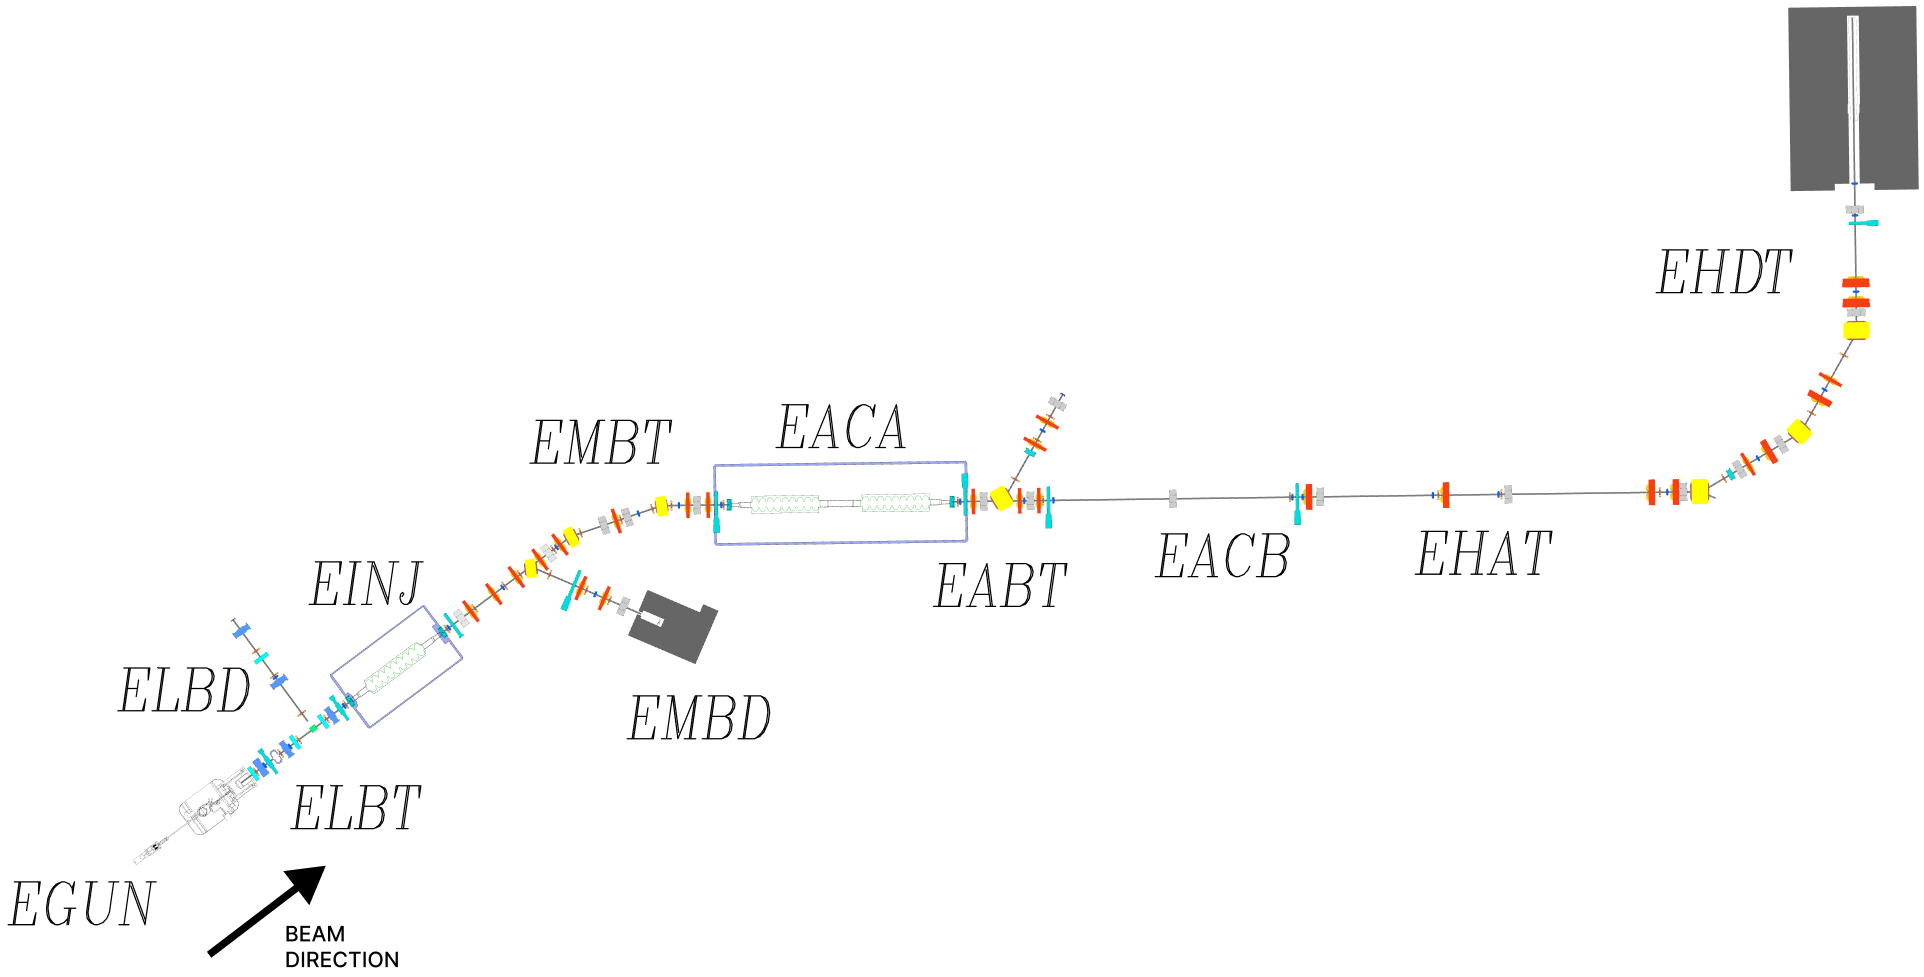
\includegraphics[width=\textwidth]{images/beam_line4.png}
    \caption{Schematic layout of the e-Linac from the electron gun to the high energy dump.}
    \label{fig:layout}
\end{figure}
     The transverse beam profile serves as a critical window into the behavior of particles within an accelerator beam at specific longitudinal points, providing intricate details about their spatial distribution and momentum. This profile plays a pivotal role in evaluating and assessing the anticipated characteristics of the beam \cite{storey2011view}. Within the e-Linac, dedicated diagnostic boxes host View Screens—beam profile monitors that emit scintillation photons upon interaction with electrons. These emitted photons are captured by a camera and converted into digital data, resulting in a comprehensive visual representation of the electron beam's cross-sectional layout and distribution. This report explains the technology and methodology implemented at TRIUMF to ascertain the transverse beam profile for the e-Linac. Furthermore, it outlines the development of an automated pipeline designed to systematically gather, analyze, and compare beam sizes derived from experimental data with the theoretical predictions generated by the envelope code TRANSOPTR \cite{baartman2016transoptr}.

\newpage
\section{Theory}

\subsection{Transverse Beam Profile}

A high number of particles, which are congregated together are known as a bunch. To describe a bunch in a machine, a co-moving coordinate system, defined by $x$, $y$ and $z$, that propagates along the design orbit $s$, is used. The design orbit describes the path of the reference particle. Not every particle has the same property as the reference particle. Along the design orbit $s$ is also the longitudinal bunch direction $z$. The orthogonal plane perpendicular to the $z$ axis is known as the transverse plane, and it is defined by the $y$ and $x$ axes. Figure \ref{fig:2} provides a visual representation of the beam, transverse plane, and coordinate system.
    
\begin{figure}[h!]
    \centering
    
    \begin{tikzpicture}
        %draw some ellipses for the cutted 3D body;
        \draw[thick,fill = red!75] (0,2) arc(90:270:4cm and 2cm);
        \draw[thick,fill = red!75] (0,0) ellipse (1cm and 2cm);
        \begin{scope}[transform canvas={rotate=20}] %this transforms the full ellipse
            \shade [top color=white, bottom color=red!75] (-1.7, 1.9) ellipse (1.2cm and 0.25cm);
        \end{scope}
        
        %draw a pararalelogram 
        \draw[fill = green!20, opacity=0.5] (-3,-4.5) -- (2,-2) -- (2,5) -- (-3,2.5) -- (-3,-4.5);
        
        %draw the main coordinate system axes
        % \draw[thick,-stealth] (0,0) -- (5,0) node[anchor=north east]{$s$};
        \draw[thick,-stealth] (0,0) .. controls (3,-0.25) and (4.5,-0.5) .. (5,-1) node[anchor=north east]{$s$};
        \draw[thick,-stealth] (0,0) -- (2.5,0) node[anchor=south east]{$z$};
        \draw[thick,-stealth] (0,0) -- (0,2.5) node[anchor=north west]{$y$};
        \draw[thick,-stealth] (0,0) -- (2,1) node[anchor=south west]{$x$};
        
        %node for explanation
        \node[rotate around={27:(6,-2)}] {Transverse plane}; 
        % \begin{scope}[transform canvas={rotate=27}] %this transforms the full ellipse
        %     \node[anchor=west] at (-3,-3) {Transverse plane};
        % \end{scope}
    \end{tikzpicture}  
    \caption{Bunch with co-moving coordinate system ($x, y, z$) on design orbit $s$.}
    \label{fig:2}
\end{figure}

The transverse plane contains information about the particles' position and deviation from the reference particle. The $x, y$ position space belongs to this plane, representing the transverse projection of a particle's position for a given $s$-value, where each $s$ value corresponds to a physical location in the beamline. The particle distribution in this space resembles an elliptical shape.

To completely describe the particle's motion, it is also necessary to have information about their velocities. The transverse phase space contains this information, and it is defined by projecting the position and momentum vectors in the transverse plane. As before, the particle distribution shape in this space is elliptical in nature but differs in that the area of the surface that contains all the particles is invariant. This means that no matter the locations in the beamline the ellipse could have different aspect ratios or tilts, but the area will remain constant. This area is known as beam emittance $\epsilon$ and its conservation constitutes a fundamental parameter that defines the quality of the beam.

In its simplest definition, transverse beam profiles are histograms that represent the number of particles in a beam as a function of transversal position. In other words, they are the result of projecting the two-dimensional position space introduced before, along a respective axis. In the case of a continuous distribution, a two-dimensional density function expressing the transverse position of particles in the beam $i(x, y)$ can be defined as follows: 
    
\begin{gather} 
\mathrm{Profile}_{H}(x) = \int_{-\infty}^{\infty} i(x, y)\,dy \label{equ:1}\\ 
\mathrm{Profile}_{V}(y) = \int_{-\infty}^{\infty} i(x, y)\,dy \label{equ:2}.
\end{gather}

For real cases, the limits of integration will be reduced to the size of the cavity. Now, assuming that the particle distribution resembles a Gaussian nature, the density function can be expressed as : 

\begin{equation} 
i(x, y) = \frac{N_{o}}{2\pi\sigma_{x}\sigma_{y}}e^{-(\frac{x^{2}}{2\sigma_{x}^{2}} + \frac{y^{2}}{2\sigma_{y}^{2}})}  \label{equ:3}
\end{equation}

and replacing \ref{equ:3} in \ref{equ:1} and \ref{equ:2}, the following is obtained
\begin{gather}
\mathrm{Profile}_{H}(x)= \frac{N_o}{\sqrt{2\pi}\sigma_{x}} e^{-\frac{x^{2}}{2\sigma_{x}^{2}}} \\
\mathrm{Profile}_{V}(y)= \frac{N_o}{\sqrt{2\pi}\sigma_{y}}e^{-\frac{y^2}{2\sigma_{y}^{2}}}.
\end{gather}  

\subsection{Statistical approach to define beam transversal profile}
Statistical quantities are fundamental in describing the ensemble behavior of particles that constitute a beam.  They offer a means to encapsulate the ensemble properties of the beam, playing a crucial role in analyzing the dynamic evolution of parameters such as beam size. At its core, the covariance matrix emerges as a key mathematical construct, providing information about the spread and correlations of position or momenta between different particles within the beam. In terms of accelerator physics language, this matrix is often known as beam matrix, or sigma matrix and in a 2-dimensional system can be represented by 

\begin{equation} 
\Sigma = \begin{pmatrix}
\sigma_{11}  & \sigma_{12} \\
\sigma_{12}  & \sigma_{22} \\
\end{pmatrix}
\end{equation}

Where $\sqrt{\sigma_{11}}$ is the RMS beam size, $\sqrt{\sigma_{22}}$ is the RMS beam divergence, and $\frac{\sigma_{12}}{\sqrt{\sigma{11} \sigma{22}}}$ is the statistical correlation between the two-phase space variables. The beam evolution across points A and B in the beamline can be determined using the beam matrix and introducing a transfer matrix $\bold{M}$ as follows 

\begin{equation} 
\Sigma_{B} = \bold{M} \times \Sigma_{A} \times   \bold{M}^{T}
\end{equation}
 The transfer matrix accounts for the optics operations that particles undergo as they propagate through an optical system, describing linear transformations of the particle coordinates and momenta as they travel through magnetic and electric fields. Another important quantity of interest is the geometrical RMS beam emittance which is proportional to the area of the distribution in phase space and is given by 
\begin{equation} 
\epsilon = \sqrt{det (\Sigma)}
\end{equation}

\section{Beam Diagnostics Systems}

Beam diagnostics play a crucial role in the design of the e-Linac. They allow the user to measure beam properties necessary for the initial beam setup and to verify that the systems behave as expected. Multiple diagnostic boxes have been installed along the e-Linac, distributed across low, medium, and high energy sections. Each box contains a set of hardware components designed to ascertain crucial beam characteristics, including beam position, transmitted beam current, transverse beam profile, beam halo, emittance, beam momentum, and energy spread, among others.   

The methodologies employed to identify the beam properties can be classified as intercepting and non-intercepting \cite{storey2011view}. Intercepting methodologies encompass direct interaction between an object positioned within the beam's trajectory and the particles constituting the beam. This approach is destructive since it obstructs the beam from propagating, but it provides the best results when it comes to identifying beam positions and profiles. Non-interacting methods are the opposite and refer to techniques where the particle's trajectory as it propagates downstream is not disturbed. In the e-Linac intercepting methods are used to identify transversal beam profiles which is the principal interest of this report and will be discussed in the following section. 
    
\subsection{View Screens}
    
View Screens (VS), often known as Beam Profile Monitors, are intercepting devices that produce a two-dimensional image of the beam intensity as a function of position. They consist of beam targets, which emit electromagnetic waves (photons) as beam particles pass through them, and an imaging system to construct images from the emitted light. There is a linear proportionality between the intensity of the light emitted by the beam targets and the beam particle density, resulting in higher intensity in regions of greater particle concentration within the spatial domain. 
    
For low-current beam measurements, the prevalent choice of beam target involves scintillation screens \cite{storey2011view}. These screens emit scintillation light when beam particles interact with them. The emitted light closely originates from the point where the beam particle passes through the screen, creating a light pattern on the screen that matches the density profile of the beam. The emitted light is then collected and focused onto a CCD sensor for image capture through the optical imaging elements located within the camera box. 
    
The material used for the screens in the e-Linac is a very fast scintillator, named YAG:Ce (Cerium doped Yttrium Aluminum Garnet), which has a decay time of approximately 70 $ns$, and emission spectrum peaked at a wavelength of 550 $nm$ \cite{storey2011view}. Figure \ref{fig:5} provides a visual representation of the main elements that compose the View Screens design including the different available beam targets and imaging system. 

A total of 15 View Screens have been installed and commissioned along the length of the e-Linac. Each of them has a corresponding unique name that provides an intuition about its location as well as a unique $s$ value that identifies its longitudinal location with respect to the starting point of the e-Linac's beamline. Appendix \ref{appendix:VS_NAME_S} tabulates the names and s position for all 15 VS for easy access.

\newpage    
\begin{figure}[!h]  
    \centerline{\ 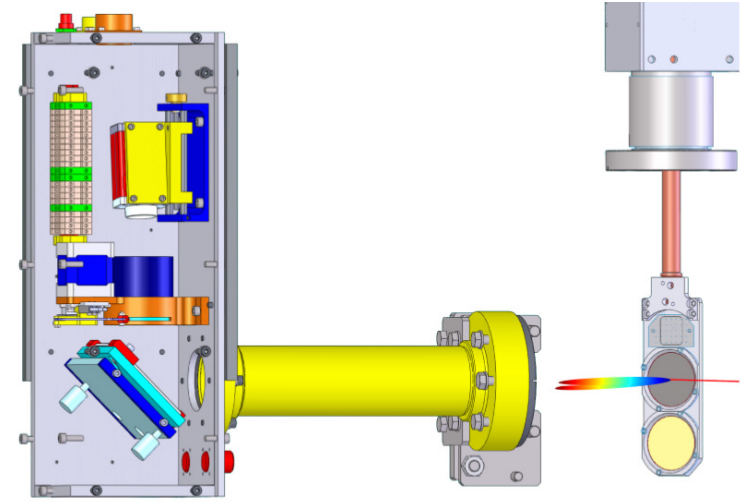
\includegraphics[width=\linewidth]{images/viewscreen_system.png}}
    \caption{Schematic diagram of the layout of the e-Linac View Screen diagnostic system. The image shows the target holder to the right of the picture, containing an OTR target mounted in the middle position and the YAG:Ce screen at the bottom, and the camera box to the left. }
    \label{fig:5}
\end{figure} 

\subsection{Control System and Software}

Experimental Physics and Industrial Control System (EPICS) is a set of open-source software tools and applications designed to develop and implement distributed control systems that provide full operating control over complex devices \footnote{https://docs.epics-controls.org/en/latest/}. The e-Linac control and monitor system has been implemented in EPICS, and it allows the user to have full control over devices along the beamline through an intuitive user interface that can only be accessed from the control room. 

From a high-level perspective, EPICS is a toolset that allows the creation of servers and client applications. Servers are in charge of providing data access (reading or writing) through IOCs (input-output controllers) and clients use these servers to interact with hardware components. In its simplest sense, IOCs can be thought of as stand-alone computers whose responsibility is to communicate with a sub-section of the equipment comprising the e-Linac. In EPICS, I/O devices are treated as data entities that describe a single aspect of the process or device under control and are represented by process variables (PVs). A PV could represent a particular attribute in the equipment such as power supply current and voltage, solenoid currents, and others.

All the elements that constitute the diagnostic systems for View Screens can be accessed and adjusted through their dedicated PVs. This ability to manipulate the state of VSs will be leveraged to create an automation system that facilitates the collection and processing of VS images by creating a logical procedural sequence of PV value changes that translate in specific orders to the hardware, producing a desired outcome. Appendix \ref{appendix:VS_PV} shows all the PVs required to have complete control over the View Screens.
     
It is important to note that external applications do not have direct access to change the state of the machine, meaning set or get PVs, but rather they have to communicate through API endpoints managed by High-Level Application (HLA) \footnote{More information about HLA applications can be found at https://hla.triumf.ca/}. In particular, Jaya is an HLA designed to be the gate between the communication of external applications and EPICS. It provides multiple endpoints to set/get PVs and perform other activities, documentation about it can be found in its respective Gitlab repository\footnote{ Jaya's repository can be found at https://gitlab.triumf.ca/hla/jaya}.  

\section{Calculation Beam Transverse Profile}

Determining the RMS of the transverse particle density distribution in the position domain provides enough information to describe the longitudinal beam's propagation, and are the key values that need to be determined.
    
Since pixel intensity in images captured with the VSs diagnostic systems is proportional to the flux of particles interacting with the screen at defined spatial positions, calculating the RMS in the pixel domain is equivalent to calculating it in the position domain, and a mapping relation can be used to transform from pixels to distance. For each individual VS a proportionality value between pixels and millimeters was measured, and it is tabulated in Appendix \ref{appendix:VS_NAME_S}. 

To determine the RMS values of the pixel intensity distribution, a custom processing image package \footnote{ This package was originally developed by Tate McCartney, and has undergone slight adjustments since his last version. Documentation about the package can be seen in the GitLab repository at https://gitlab.triumf.ca/hla/student-projects/beam-profile-vs} has been internally developed at TRIUMF. From a high-level perspective, the package functionality is simple, it takes as input a VS image, performs multiple discrimination methods to eliminate pixels that correspond to nonbeam artifacts, fits an ellipse to the beam data, and returns the RMS values and centroids for the x and y distributions in pixels and millimeters. Figure \ref{fig:6} shows an input image example for ELBT$\_$VS2 as well as a surface plot of the same image where the z-axis represents pixel intensity. 
     
An essential feature of the package is its ability to discriminate nonbeam pixel artifacts. These artifacts encompass any pixel within the input image that does not correspond to the light generated by interactions between beam electrons and the scintillator screen. There are multiple reasons why these artifacts are produced but primarily they are a result of light reflected by the VS frame or dark current. If these nonbeam pixels are not properly discriminated biases are introduced to transverse distribution and misleading RMS values are obtained.

\begin{figure}[!h]  
    \centerline{\ 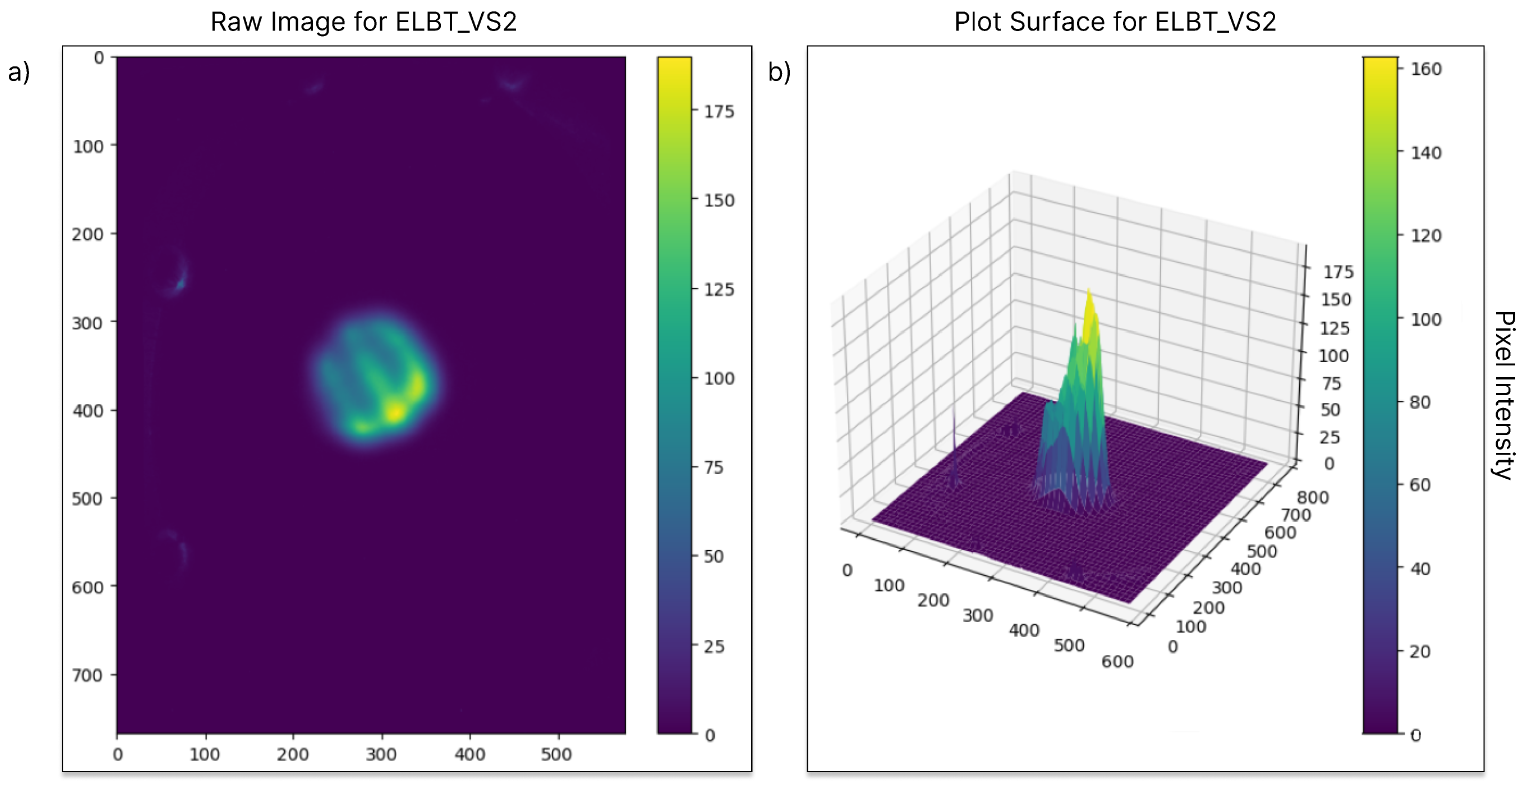
\includegraphics[width=\linewidth]{images/example_vs_output.png}}
    \caption{Sample input image for ELBT$\_$VS2. a) Raw VS Image, showing beam pixels in the middle and artifacts created by light reflected in the VS frame. b) Plot surface for the same input image where the z-axis represents the pixel intensity.}
    \label{fig:6}
\end{figure} 
    
\subsection{Nonbeam pixel artifacts}
    
Distinguishing between nonbeam and beam pixels can be challenging due to the overlap in intensity values. This is particularly true when it involves discerning which pixels define the outer beam profile. The view screen processing package incorporates a series of sequential methods designed to intelligently identify nonbeam data and discriminate it. However, before digging deeper into how these methods work, it is important to understand why nonbeam pixels appear in the image. 
    
As mentioned in the previous section, there are two main reasons for the existence of nonbeam pixel artifacts, light reflected from a component of the VS and dark current. The first one is quite intuitive, some of the scintillation light emitted in random directions is reflected back by an element in the VS, such as the screen frame. If this light is reflected with the proper angle it will enter the camera box, pass through the focusing elements, and hit the CCD. Given that these reflection events are inherently random in nature and the pixel intensity is related to the rate of photons-per-time-unit that hit a specific section of the CCD, it will be expected that observed pixels created due to this reason have a low intensity compared to beam pixels. These artifacts are especially noticeable for VS with observable frames which are EGUN$\_$VS1, ELBT$\_$VS0, and ELBT$\_$VS2.

On the other hand, another source contributing to nonbeam pixels is dark current. The e-Linac uses SRF cavities, which apply variable electromagnetic fields to accelerate electrons along the propagation axis. These fields induce field emissions from the accelerator walls, resulting in the flow of electron currents. If these electrons are captured in phase along the beamline, they will gain kinetic energy and produce an undesirable background dark current (hence the name) that interferes with the primary electron beam. In a general sense, any current of electrons present in the beamline when the electron gun is turned off and the RF Source is turned on is considered to be a dark current. Effects due to dark current in VS images are maximized in screens that follow acceleration modules (EINJ and EACA) such as EMBT$\_$VS0, EMBT$\_$VS4, EABT$\_$VS1, and EABT$\_$VS2. Figure \ref{fig:7} shows binary pictures that display nonbeam and beam pixels, demonstrating the biases introduced by light reflection and dark current.  

\begin{figure}[!h]  
    \centerline{\ 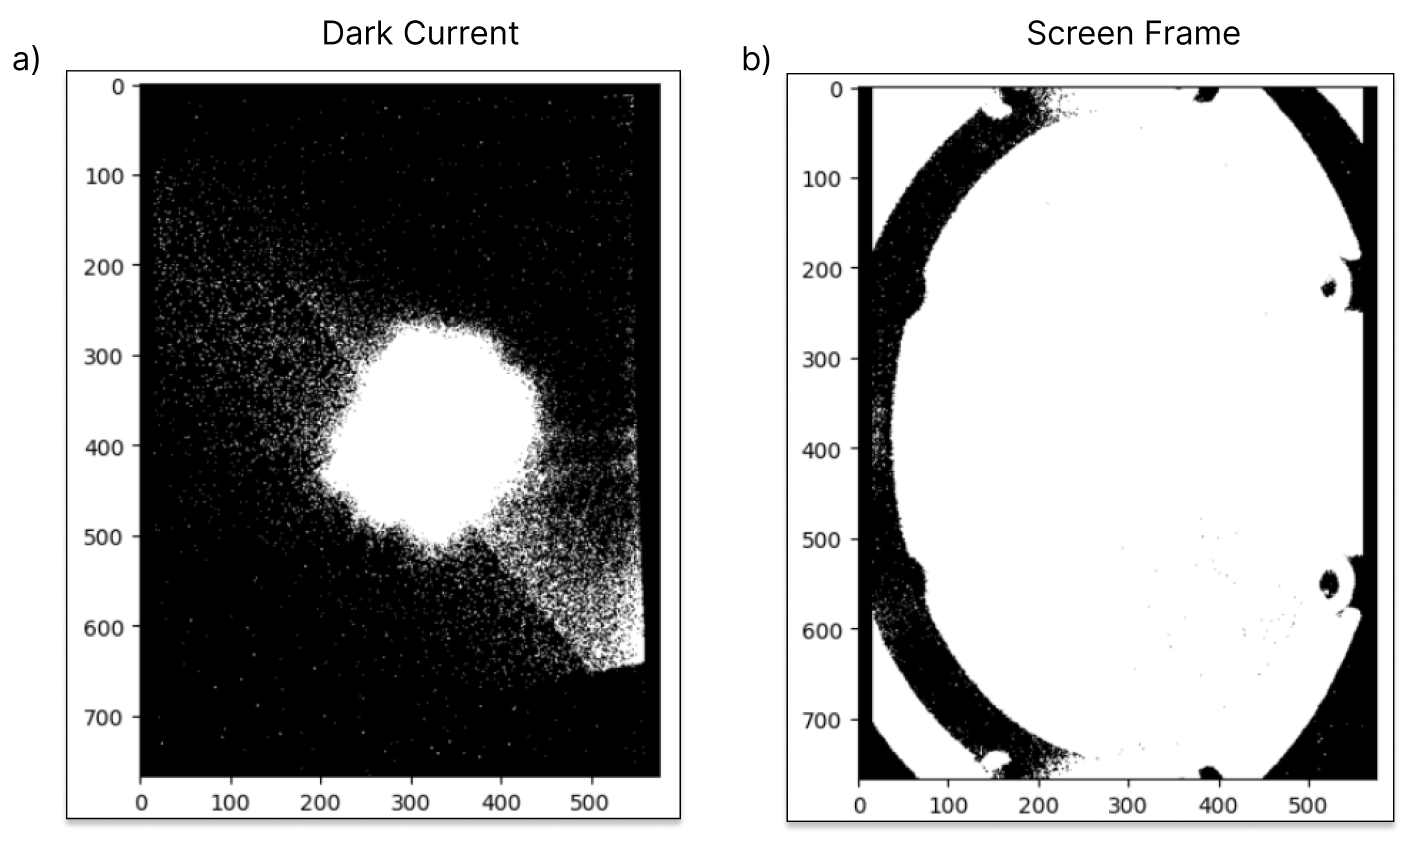
\includegraphics[width=\linewidth]{images/example_nonbeam_pixel_aberrations.png}}
    \caption{a) Binary image for EMBT$\_$VS4 showing off center pixels created due to dark current. b) Binary image for EGUN$\_$VS1 showing the nonbeam pixel artifact due to light reflected in the VS frame. For a) and b) dark regions in the image correspond to intensities equal to zero and white to intensities greater than zero.}
    \label{fig:7}
\end{figure} 


\subsection{Discrimination nonbeam data}

The core of the viewscreen processing package consists of image manipulation methods tailored primarily to identify and eliminate unwanted pixels. These types of pixels are produced by different mechanisms (as commented previously), but they exhibit some common traits that are utilized to differentiate them from beam data. One of these characteristics is their sparsity in the image domain. In other words, they often manifest as dispersed random patterns of points across the image, encircling a bright cluster of pixels that correspond to the beam. This does not hold entirely true for pixels originating from light reflected by VS components,  like the frame, as they also form pixel clusters near the image edges. However, despite this, it is always possible to exploit the sparsity of the nonbeam signal to identify and remove small solitary islands of pixels.

A second important distinction is the pixel intensity. Considering that pixel intensity is proportional to the number of photons reaching the CCD within a defined time interval, and that the highest photon flux arises from the scintillation light generated by beam electrons, it is logical to anticipate that beam pixels would exhibit the highest intensity among all the pixels constituting the image. While this assertion holds valid for the majority of beam pixels, there are exceptions. Instances occur where pixels delineating the edges of the beam signal demonstrate intensity levels similar to the nonbeam artifacts present in the image., e.g. when there is a significant presence of dark current.   

The algorithms that compose the package leverage both the sparsity and pixel intensity difference to discriminate nonbeam data before trying to calculate the RMS of the distribution. There are four sequential methods written for this purpose: \texttt{apply$\_$frame$\_$mask}, \texttt{safe$\_$subtraction}, \texttt{threshold$\_$from$\_$nonzero} and \texttt{remove$\_$small$\_$objects}. There are other methods contained in the package that do not manipulate the image but can determine oversaturation:  \texttt{detect$\_$overexposure} and \texttt{detect$\_$exposure$\_$within$\_$boundary}. Figure \ref{fig:8} shows a high-level example of the input and output of the package as well as intermediate steps.
    
\begin{figure}[!h]  
    \centerline{\ 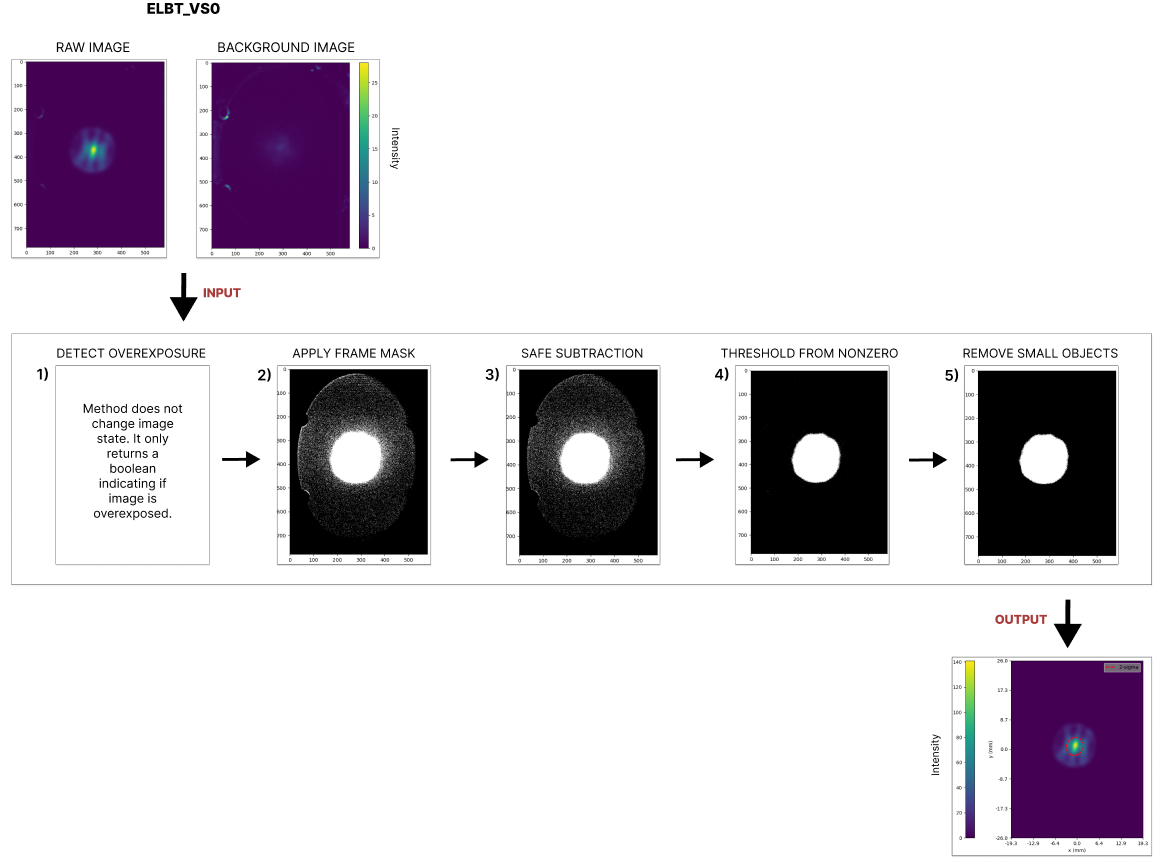
\includegraphics[width=\linewidth]{images/processing_pipeline.png}}
    \caption{ Image shows an input example of beam on and off images for ELBT$\_$VS0 to the viewscreen processing package. The package executes a sequence of nonbeam discrimination steps, calculates the RMS values of the pixel distribution, and returns an output image displaying the ellipse that corresponds to the 2RMS value. Note, that images displayed during intermediate steps are shown in binary form, where pixels are black if the intensity is zero, otherwise white. This choice enhances the clarity of each method's effects.}
    \label{fig:8}
\end{figure} 
\newpage
    
\subsubsection{Remove Frame Mask}

There are three VSs (EGUN$\_$VS1, ELBT$\_$VS0, and ELBT$\_$VS2) whose frames are distinctly visible in the collected images. The position of these frames remains unchanged, and through multiple measurements, parameters of ellipses that enclose both the frame and any screws have been empirically determined. This method simply uses these parameters \footnote{The ellipse parameters can be found in the config.json file of the respective project.} to generate discrimination masks. Upon overlaying these masks onto the image, they effectively identify and eliminate all pixels corresponding to the frames and screws by setting them to zero. Note that this method returns without modifying the image for screens whose ellipse parameters have not been defined. Figure \ref{fig:9} provides a visual representation of how this method behaves for an EGUN$\_$VS1 sample image.
    
\begin{figure}[!h]  
    \centerline{\ 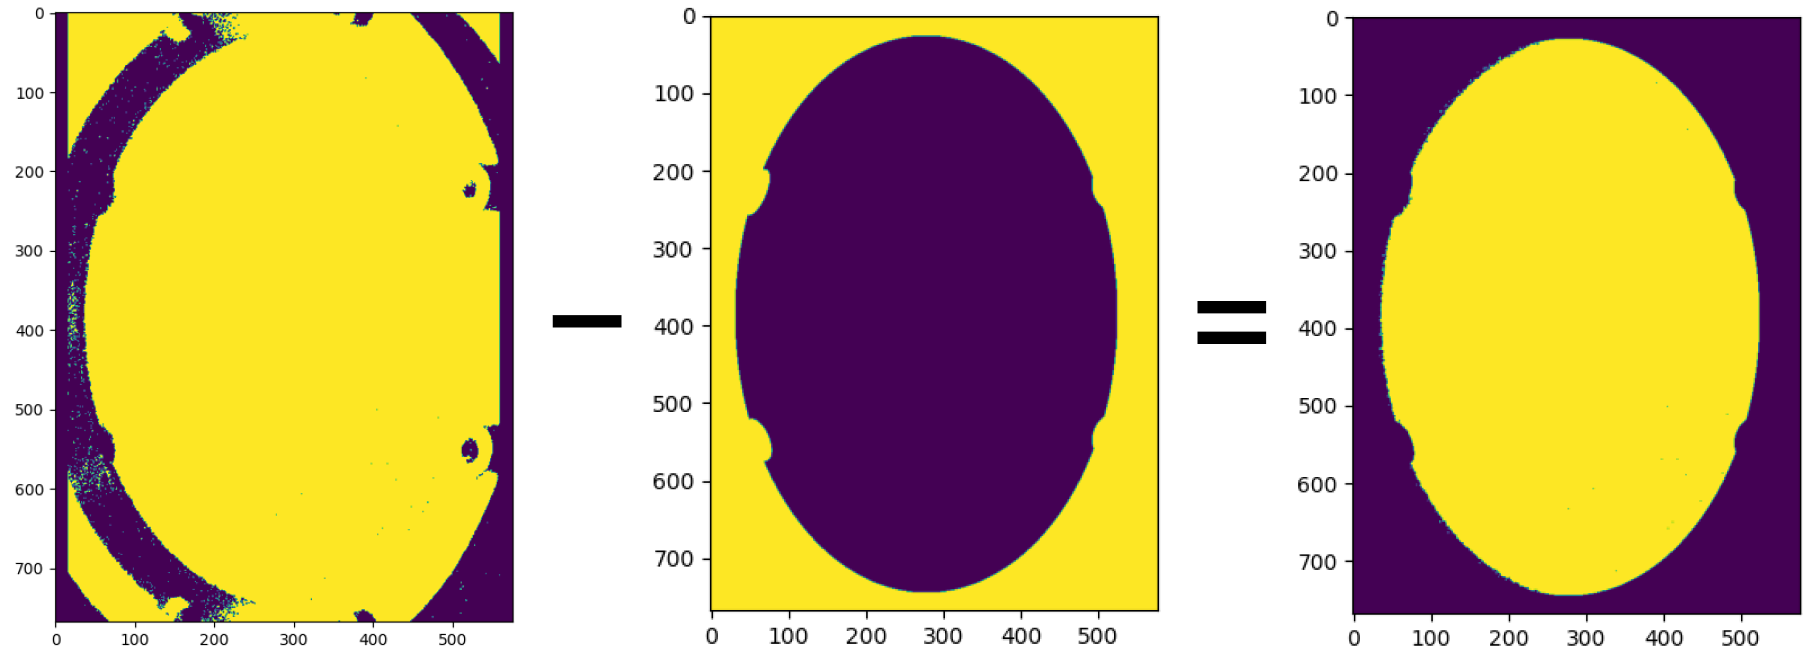
\includegraphics[width=\linewidth]{images/first_step.png}}
    \caption{Visual representation of \texttt{apply$\_$frame$\_$mask} execution. The first image to the left represents the raw binary image for EGUN$\_$VS1, where yellow corresponds to pixels greater than zero. The middle image illustrates the mask derived from empirically measured ellipsoid parameters specific to this VS. Finally, the image on the right demonstrates the outcome of the method after overlapping the mask to the input image and setting to zero all overlap pixels that are not zero. Note that in this figure the minus does not represent subtraction.}
    \label{fig:9}
\end{figure} 

\newpage
\subsubsection{Remove Background}

Artifacts originating from dark currents present a challenge when discerning them from beam data, because of their closely matched pixel intensities and clustered formations within the captured images. A simple yet effective method to reduce the intensity of these pixels, if not entirely eliminating them, is to capture a \say{beam-off} image (background) immediately after acquiring the \say{beam-on} image, and subtracting both images. This is the essence of the \texttt{safe$\_$subtraction} method, it simply subtracts both images and adds an extra condition to avoid negative pixels.

Ideally, this method should be capable of eliminating all traces of artifacts present in the background image, but this could not be further from the truth. It has been observed that even after subtraction, residuals of background pixels are left in the beam-on images, although with a significant decrease in intensity. The most intuitive explanation is that there is a dependency between the beam status and dark current. Turning the beam on or off also affects the dark current state, resulting in a mismatch between beam on and off images. These effects can be mitigated by minimizing the time interval between image collections.

It is also important to notice that if no beam-off image has been provided, the beam-on image is not modified, and the method simply returns. Figure \ref{fig:10} provides a visual representation of the effectiveness of reducing nonbeam pixels by this method.

\begin{figure}[!h]  
    \centerline{\ 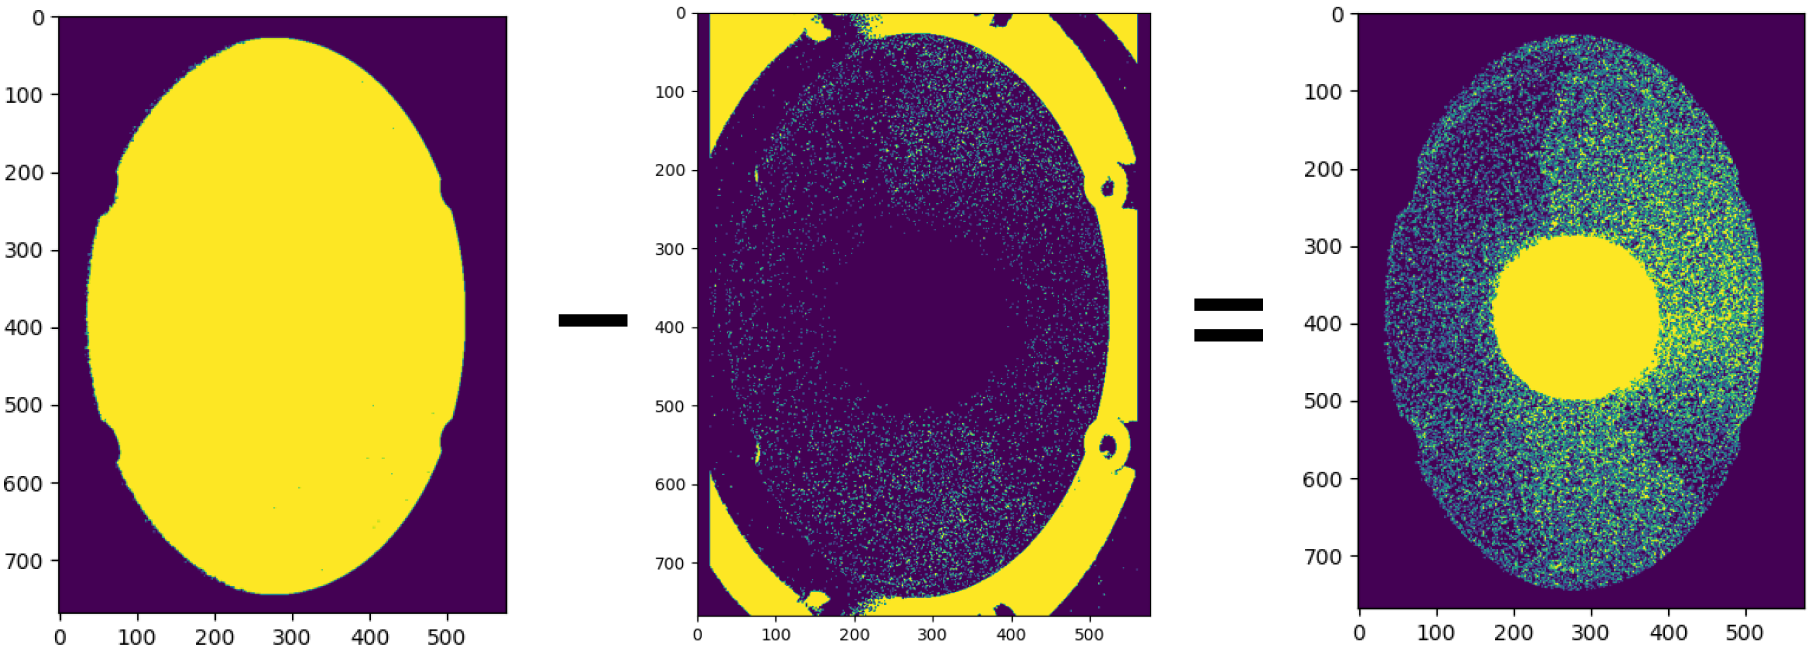
\includegraphics[width=\linewidth]{images/second_step.png}}
    \caption{Visual representation of \texttt{safe$\_$subtraction} execution. The sequence of images, progressing from left to right, illustrates the process for EGUN$\_$VS1. The initial image shows the input image after the removal of the VS frame. The middle image contains the background image (beam off), and the final image displays the outcome following the background subtraction.}
    \label{fig:10}
\end{figure} 
\newpage

\subsubsection{Remove Small Objects}

As previously discussed, an anticipated characteristic of nonbeam pixels is their sparsity. This means that they often manifest as isolated, small discontinuous pixel chunks. The challenge at hand is to identify and subsequently remove these dispersed, solitary pixel regions from the image by setting their values to zero. This is where \texttt{remove$\_$small$\_$objects} method shines. It is basically a wrapper for \texttt{skimage.morphology.remove$\_$small$\_$objects} \footnote{Documentation about this method can be found at \url{https://scikit-image.org/docs/stable/api/skimage.morphology.html}}, which takes two key parameters $min\_size$ and $connectivity$. The first one, $min\_size$, specifies the minimum size or area that an object must have to be kept, and the latest one, $connectivity$, refers to the type of connectivity used to determine if pixels are connected or not. Figure \ref{fig:11} provides an example of how this method behaves. 
    
\begin{figure}[!h]  
    \centerline{\ 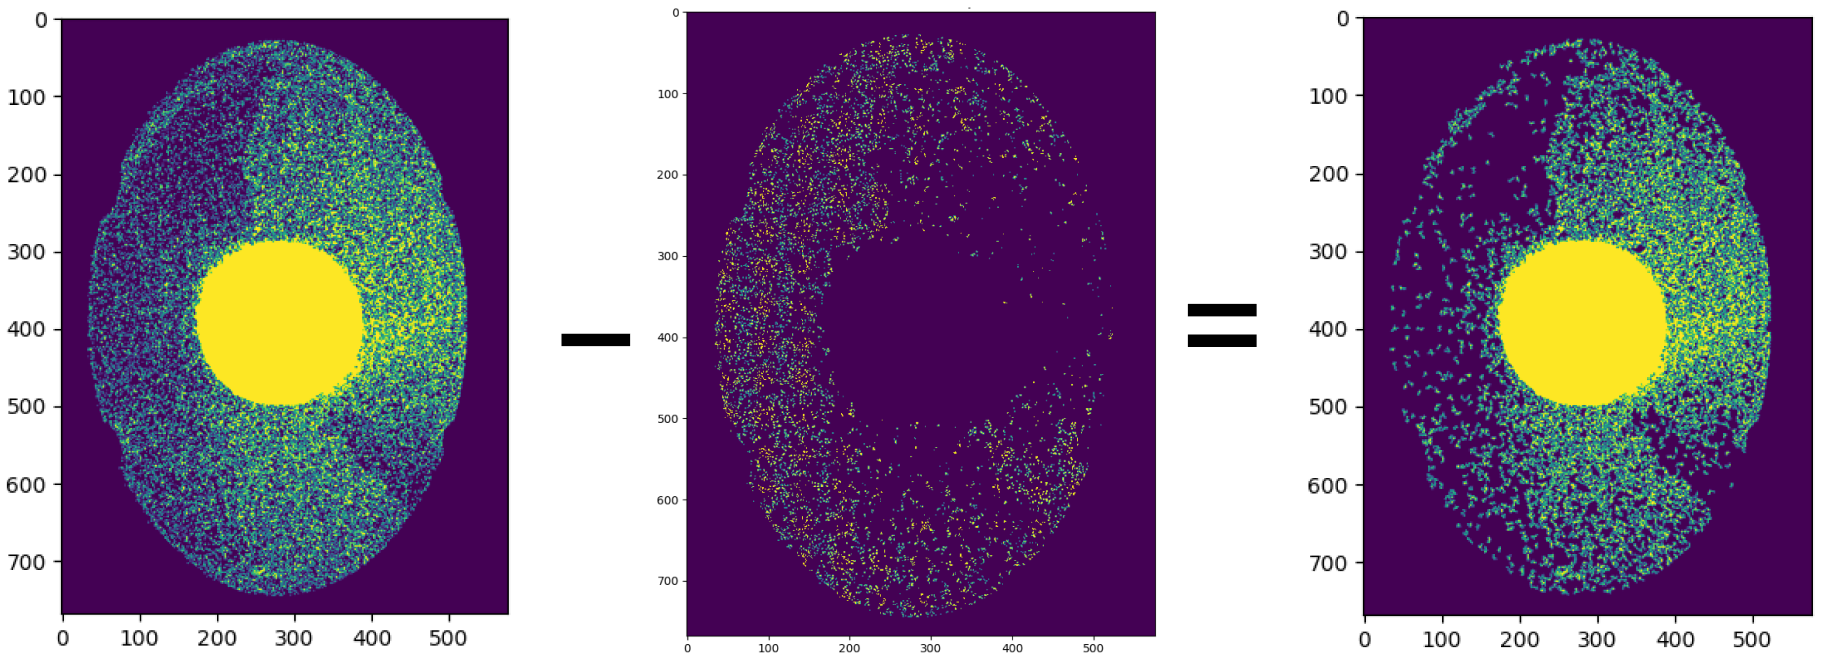
\includegraphics[width=0.95\linewidth]{images/third_step.png}}
    \caption{Visual representation of \texttt{remove$\_$small$\_$objects} for a sample input image of EGUN$\_$VS1 after subtracting the background. From left to right, the first image corresponds to the raw image, the middle shows the identified small components and the last one is the final output.}
    \label{fig:11}
\end{figure} 

\newpage
\subsubsection{Remove Below Threshold}

This is an intensity discrimination method, named \texttt{threshold$\_$from$\_$nonzero}, that attempts to identify an ideal intensity cutoff threshold value. Any pixel with an intensity less than the threshold is set to zero. For optimal performance, this method must be applied after background discrimination, so the pixel intensity difference for beam and nonbeam data is maximized. It also provides better results if applied before the \texttt{remove$\_$small$\_$objects} method, since it increments the number of small nonconnected components in the image.

The effectiveness of this method depends on identifying a suitable discrimination threshold that efficiently eliminates a substantial amount of nonbeam data. The logic to identify the best threshold value follows the next steps:
\begin{enumerate}
    \item Fit a 2D Gaussian to the image intensity distribution to identify a confidence region defined by $6 \sigma$ ellipse. Anything outside this ellipse will be considered to be nonbeam data. 
    \item Look for the highest pixel intensity $n$ outside the ellipse. If there exist pixels with intensity $n-1$ also outside the ellipse then keep $n$ otherwise look for the second highest. Continue this process for lower order intensities until an appropriate intensity n that meets the requirements is found, and name it as MAX$\_$CONTINUOUS.
    \item If the percentage of non-zero pixels in the region outside the ellipse is less than five percent then no threshold discrimination is applied. Otherwise, check if the percentage is greater or equal to fifty percent and set the threshold equal to MAX$\_$CONTINUOUS. If it is between three and fifty percent then set the threshold to be one \footnote{This value is purely empirical, and it was determined after looking at multiple VS images.}.   
\end{enumerate}
    
Once an ideal threshold has been identified, any pixel below it is set to zero. It is important to highlight that when executing this method for different VS images a threshold value of one is frequently observed. Figure \ref{fig:88} shows an example of applying this method to a VS image.

\begin{figure}[!h]  
    \centerline{\ 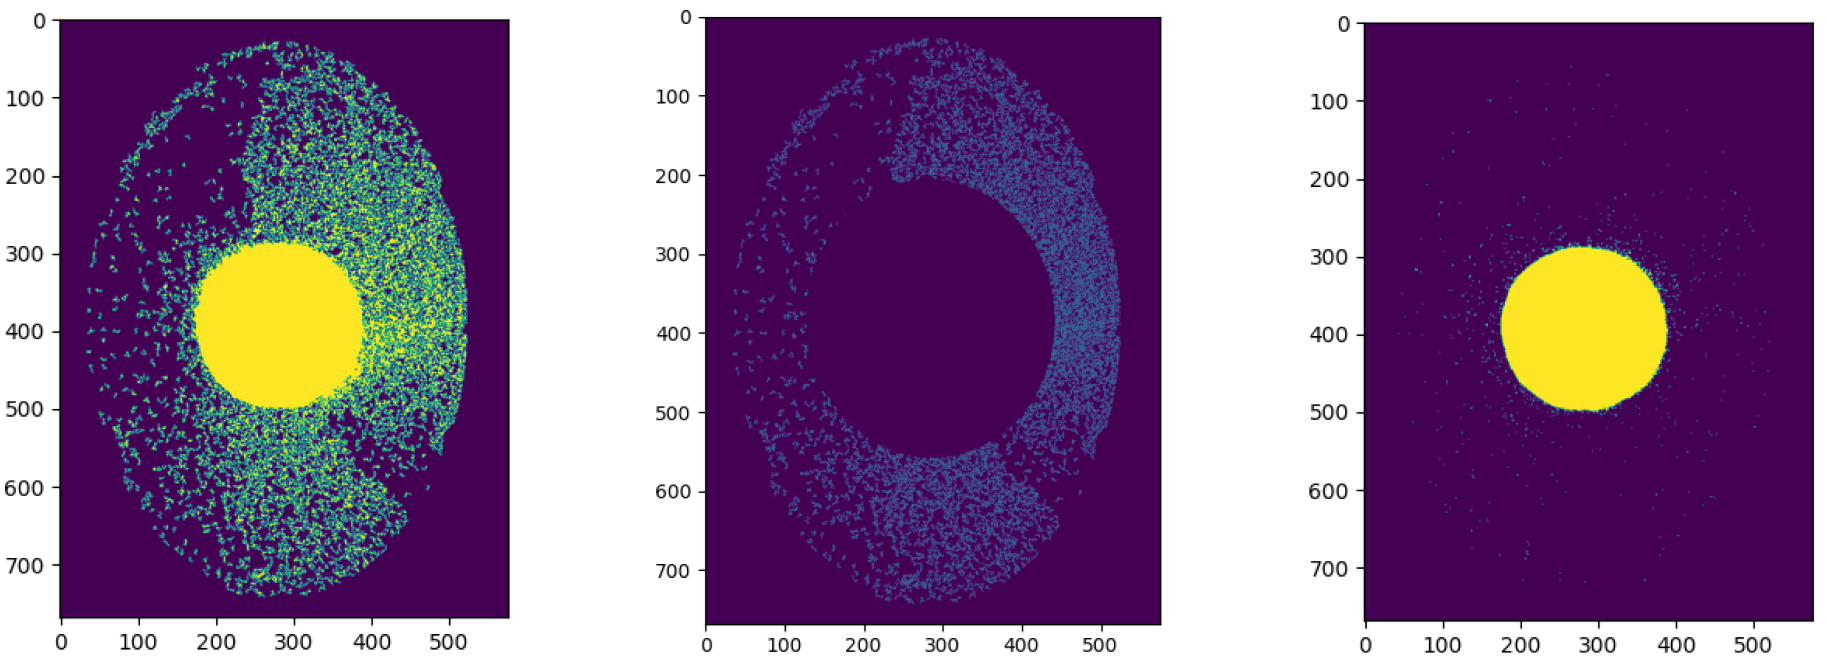
\includegraphics[width=\linewidth]{images/last_step.png}}
    \caption{Visual representation of \texttt{threshold$\_$from$\_$nonzero} applied to a sample input image for EGUN$\_$VS1 after executing \texttt{remove$\_$small$\_$objects} on it. Starting from the left, the first image is the input raw image, the middle image shows the pixel region used to find a possible value for the threshold, and the last picture shows the output image. In this example, the percentage of non-zero pixels within the area shown in the middle is between three and fifty percent, and following the explanation above the respective threshold value is one.}
    \label{fig:88}
\end{figure} 

\subsubsection{Detect overexposure}

This method, named detect$\_$overexposure, does not produce any modifications to the input image but rather provides a sanity check to identify if there are any oversaturated pixels that could lead to miscalculation for the RMS. The definition of oversaturation in this method is the following if there exists two or more consecutive maximum intensity pixels (255 in the case of black and white images) in the image then it is oversaturated.

\subsubsection{Detect overexposure within boundaries}

This method, named detect$\_$exposure$\_$within$\_$boundary, is used by the automation pipeline to correctly find an acquisition time that produces an image that is not oversaturated or undersaturated. To accomplish this, the method scans the image using an $n \times n$ \footnote{Where n can be user-defined, but it defaults to 4.} matrix, progressing from left to right and top to bottom. During this scan, it computes the average pixel intensity of the pixels enclosed by the window matrix. Once the scan is completed, the maximum average pixel intensity is determined. If this maximum average falls within the interval of [150, 240] then the image is classified as perfectly saturated.   

\section{Automation View Screen Imaging Collection and Processing}

The process of collecting and processing VS images is a repetitive consistent task, and it is an ideal candidate for the development of an automated system. In fact, this is the functionality of the VS image collection and processing pipeline package \footnote{The repository for the package can be found at \url{https://gitlab.triumf.ca/hla/student-proj}}. It utilizes other HLAs to communicate with EPICS, process VS images, and compare the results with a theoretical model simulated by TRANSOPTR. Figure \ref{fig:13} gives a high-level perspective of HLAs used by the package. For instructions on how to execute the pipeline, please refer to Appendix \ref{appendix:exe_pipeline}.

\begin{figure}[!h]  
    \centerline{\ 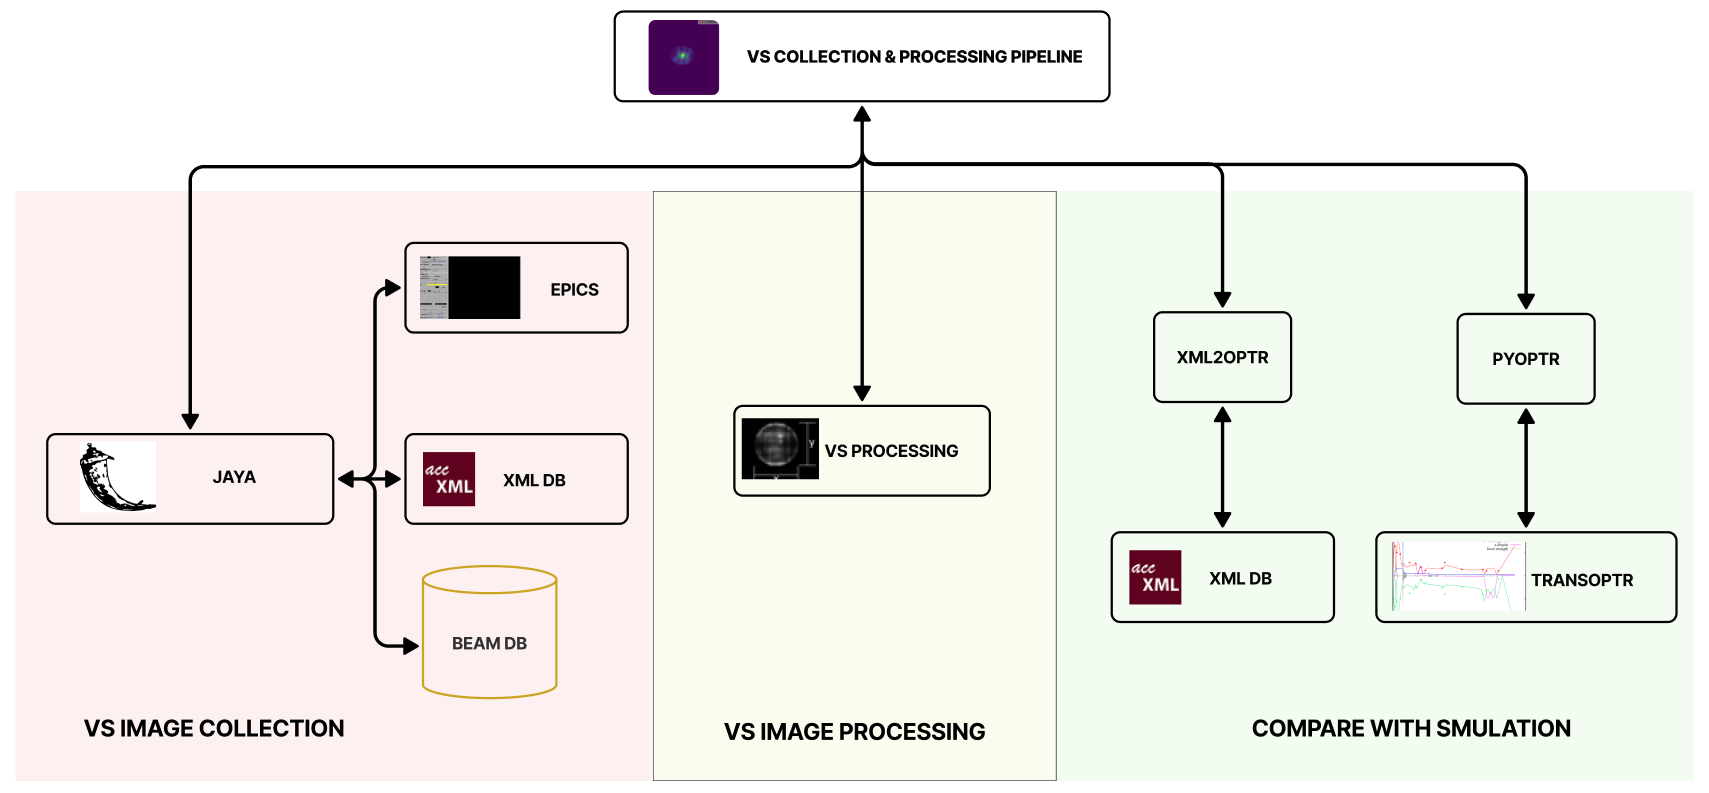
\includegraphics[width=1.13\linewidth]{images/hla.png}}
    \caption{External applications used by the collection and processing pipeline program. }
    \label{fig:13}
\end{figure} 

A complete overview of the pipeline execution logic can be summarized by looking at each of its three principal functionalities. First, it is responsible for collecting images from user-defined screens situated along a designated beampath. To achieve this, it communicates with EPICS via Jaya to perform a sequence of consecutive commands (API calls) to instruct the diagnostic system to collect VS images as needed and save them locally and in the beam database. This sequential group of calls mirrors the steps performed by an operator to set up the machine and acquire an image. It is important to note that while the collection of images is not fully automated, it operates in a hybrid mode, requiring occasional user intervention. Instances demanding user engagement during program execution include turning the beam on and off, breaking the EOECM, and resetting the interlock mechanism.
    
Second, it processes each individual image by running all four sequential discrimination methods (mentioned in the previous section) to eliminate all nonbeam nuisance and determine the 2RMS values for each positional distribution in $x$ and $y$. Depending on the options the program is executed with, the final processed image with a 2RMS ellipse overlayed on top is saved locally. For debugging purposes, the program could also be set to output a binary image of the beam before and after artifact discrimination.   

Third, it uses XML2OPTR \footnote{The respective Gitlab repository can be found at \url{https://gitlab.triumf.ca/hla/acc-utilities/xml2optr}} to create the input files needed to run TRANSOPTR (\say{data.dat} and \say{sy.f}), and PYOPTR \footnote{The respective Gitlab repository can be found at \url{https://gitlab.triumf.ca/beamphys/pyoptr}} to execute TRANSOPTR with the parameters used in the dataset collection step. It then compares the simulated beam sizes outputted from TRANSOPTR with the calculated ones. Agreement between both the theoretical and experimental values is indispensable to assess the proper functionality of the accelerator. 

The program allows for both online and offline execution. The principal distinction between both is that offline execution does not communicate with EPICS. Therefore, it does not collect VS images or save to beam DB, and it is only functional if the input images are pre-collected, and a path to them is provide. It is intended to provide an alternative execution when the user has a previous dataset collected and would like to know the RMS values and compare them with the theoretical simulation. Furthermore, there are two types of execution modes: initial conditions solenoid scan, and esnapshot. Both are available with either online or offline execution and will be discuss below. 

\subsection{Pipeline execution options}

As previously mentioned, there are two primary execution types (online and offline), along with two distinct modalities (initial conditions solenoid scan and esnapshot). To designate the execution type, a command-line argument is used when running the pipeline, as detailed in Appendix \ref{appendix:exe_pipeline}. To specify the modality and other required information, JSON input files are used. Refer to Appendix \ref{appendix:input_files} to learn more about the input files and their options.
    
\subsubsection{Initial Conditions Scan}

The initial conditions modality, defined in the program as init$\_$scan, allows the user to execute a current scan for one or more solenoids. This entitles collecting a VS image for each current value, where the user can define multiple solenoid-VS pairs by adding custom arrays of VSs and solenoids into the input file. To find a solenoid-VS pair the program looks at the longitudinal position ($s$) of the input components and creates all possible combinations that obey the following condition $s_{solenoid}< s_{VS}$. e.g. If the input list of solenoids is [EGUN:SOL1 , ELBT:SOL1] and VSs is [EGUN:VS1 , ELBT:VS0] then the match solenoid-VS pairs are [(EGUN:SOL1, EGUN:VS1), (EGUN:SOL1, ELBT:VS0)].

The currents to set in the solenoid can also be customized by adding a list of current values to the input file. Otherwise, it is required to provide the current that produces the minimum ($min\_current$) and maximum ($max\_current$) beam sizes, and the number of data points ($steps$) wanted in the current list. Then the algorithm to create the current list follows the following logic:
\begin{itemize}
    \item Defines a list ($v$) that contains $steps$ evenly spaced numbers.
    \item For each element in the list perform the following transformation $v_i = (\mid v_i \mid * v_i)^{2}$
    \item Then defined each element in the current list ($l\_curr$) as $l\_curr_{i} = min\_current + v_i * (max\_current - min\_current)$
\end{itemize} 

Once the currents and solenoids-VSs pairs have been defined, the execution starts. A VS image is collected for each current in a given solenoid-VS element. The image collected is then processed and a RMS value is obtained. It is important to know that as the program is executing, the RMS and processed images obtained are continuously saved to a respective output file and folder, ensuring that if the program runs into any difficulty and suddenly terminates the user has a backup of the information that has been calculated up that point. A detailed overview of how the program interacts with EPICS can be seen in Appendix \ref{appendix:init_exe}.

Once all VS images have been collected for a given current list, the program starts the post-processing routines. There are two defined post-processing steps: save into the beam database and execute TRANSOPTR. Save into beam DB saves all entries in the outputted JSON file into the beam database and prints the measurement ID obtained. On the other hand, to execute TRANSOPTR, the pipeline generates the input files (sy.f and data.dat) by tailoring the templates stored locally in the sofware's directory with the respective information settings used in the collection process. Following, it executes TRANSOPTR through PYOPTR and creates a plot $s$ versus RMS in $x$ and $y$. Figure \ref{fig:14} provides an example of the final image obtained. 

\begin{figure}[!h]  
    \centerline{\ 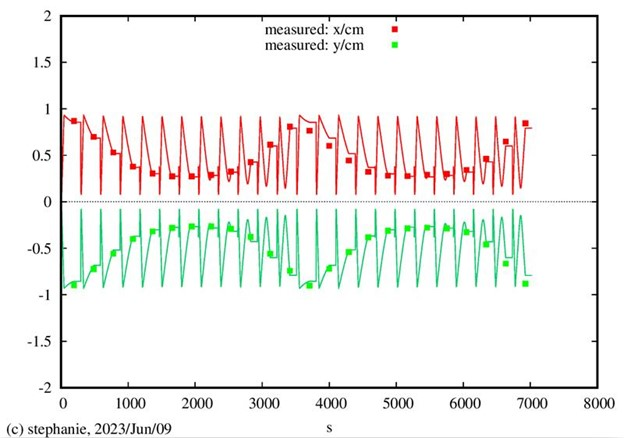
\includegraphics[width=0.7\linewidth]{images/sol_scan_transoptr_img.jpg}}
    \caption{Example of expected final output image for init$\_$scan modality, showing s $vs$ RMS cmparison, and  representing theoretical-experimental difference for beam size.}
    \label{fig:14}
\end{figure} 
    
\subsubsection{E-Snapshot}

This is the second modality supported by the pipeline, and it is defined in the program as e$\_$snapshot. Compared with the modality described previously it follows a simple execution logic. At its core it allows the user to define a set of VSs from which images are collected and processed in the same way as before. The user has the ability to enumerate all VSs that will be used in the input file or define a beampath. The VSs that conformed a given beampath can be found in the respective config.json file, and are enumerated below for completeness.  
\begin{itemize}
    \item egun-ehdt-dump: EGUN:VS1, ELBT:VS0, ELBT:VS2, EMBT:VS0, EMBT:VS4, \\ EMBT:VS5B, EMBT:VS6, EABT:VS1, EABT:VS2, EHAT:VS1, EHAT:VS4, \\ EHDT:VS0, EHDT:VS4
    \item egun-flash: EGUN:VS1, ELBT:VS0, ELBT:VS2, EMBT:VS0, EMBD:VS2
    \item egun-eabt-fc2: EGUN:VS1, ELBT:VS0, ELBT:VS2, EMBT:VS0, EMBT:VS4, \\ EMBT:VS5B, EMBT:VS6, EABT:VS1, EABT:VS2
\end{itemize} 

These beampaths exactly matched the ones defined in the XML database. In the same manner as the previous modality, while the program is under execution the processed images and RMS values are continuously being saved in the respective folder and output file. For a complete overview of how this modality executes, refer to Appendix \ref{appendix:esnapshot_exe}. 

Once all VS images have been collected the post-processing routines are executed. In the same way, there are two steps involved save in beam database and execute TRANSOPTR. Saving in the beam database behaves in the same way as before but with the difference that apart from saving VS information, extra data about the machine state is also included. Following this, XML2OPTR is used to create the input files for TRANSOPTR and PYOPTR to execute it. 

\begin{figure}[!h]  
    \centerline{\ 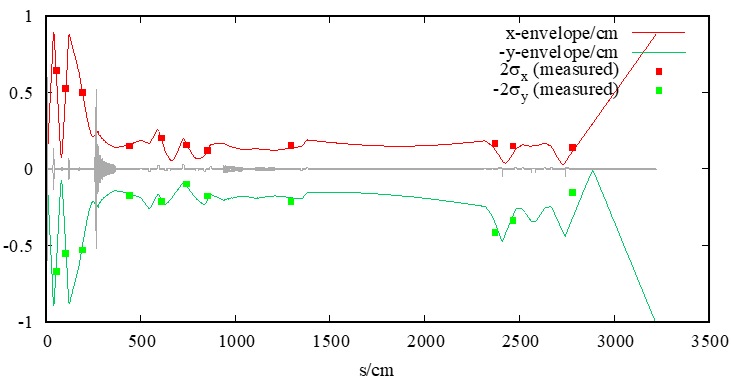
\includegraphics[width=\linewidth]{images/esnapshot_transoptr.png}}
    \caption{Example of final outputted theoretical-experimental comparison image from automation pipeline for esnapshot modality.}
    \label{fig:15}
\end{figure} 

\newpage
\section{Conclusions}

An automation pipeline that facilities the collection and processing of VS images for the e-Linac has been internally developed at TRIUMF. It is a highly customizable command line package designed with the objective of collecting, processing, and comparing transversal envelop sizes. It communicates with multiple HLAs to request operational services necessary to interact with other applications, filter out nonbeam data, calculate 2RMS values, and compare experimental beam size measurements with theoretical simulated ones generated by TRANSOPTR. 

Depending on the necessities of the user, the software has been adapted to satisfy two principal type of measurements initial conditions solenoid scan and esnapshot. The initial conditions scan is used to find the initial condition beam matrix, and it collects VS images for different current values set in a specified solenoid. The current values follow a parabolic shape in nature and contain the current that minimizes the transversal beam size. The second modality, esnapshot,  allows the user to record the machine's state by collecting multiple values of optical systems placed along a given beampath as well as VS images. The optical collected values are used by TRASNOPTR to simulated the state of the beamline and provide a theoretical model of beam RMS that can be compared with the measured one.    


\newpage
\bibliographystyle{ieeetr}
\bibliography{./bib}


\newpage
\appendix
\section{View Screen names and positions} \label{appendix:VS_NAME_S}

% \Cref{tab:vs_pv_list} Change from the non-expert. Why is any change not in the document?
Table \ref{table:vs_name} shows the name of the 15 View Screens installed along the beamline, their respective longitudinal position $s$, image output format, image dimensions, and pixel-to-mm relation.

\begin{table}[h!]
    \centering
        \begin{tabular}{ l   c   c   c   c}
            \toprule
             \multirow{2}{8em}{\textbf{VS Name}} & \multirow{2}{10em}{\textbf{Longitudinal Position ($s$) [cm]}}  & \multirow{2}{4em}{\textbf{Output format}}  & \multirow{2}{6em}{\textbf{Image Dimensions}} & \multirow{2}{4em}{\textbf{mm to pixel}} \\
             & & & \textbf{} &  \\
            \midrule
            EGUN:VS1 & 56.8540 & png & 576 x 768 & 0.0667   \\ 
            ELBT:VS0 &  105.652 & tif & 580 x 780 & 0.0667  \\ 
            ELBT:VS2 &  192.724 & png & 576 x 768 & 0.0667  \\ 
            EMBT:VS0  &  442.068 & png & 576 x 768 & 0.0322 \\ 
            EMBD:VS2  &  442.068 & png & 576 x 768 & 0.0322 \\ 
            EMBT:VS4  &  609.316 & png & 576 x 768 & 0.0322 \\ 
            EMBT:VS5B  &  743.781 & png & 576 x 768 & 0.0322\\ 
            EMBT:VS6  &  853.817 & png & 576 x 768 & 0.0322 \\ 
            EABT:VS1  &  1294.80 & png & 576 x 768 & 0.0322 \\ 
            EABT:VS2  &  1366.73 & png & 576 x 768 & 0.0322 \\ 
            EABD:VS2  &  1366.73 & png & 576 x 768 & 0.0322 \\ 
            EHAT:VS1  &  1812.45 & png & 576 x 768 & 0.0322 \\ 
            EHAT:VS4  &  2371.12 & png & 576 x 768 & 0.0322 \\ 
            EHDT:VS0  &  2466.73 & png & 576 x 768 & 0.0322 \\ 
            EHDT:VS4  &  2780.98 & png & 576 x 768 & 0.0322 \\  
            \bottomrule
        \end{tabular}
    \caption{List of VS names, longitudinal positions, image output format, image dimensions, and mm to pixels relation for all 15 View Screen installed in the e-Linac beamline.}
    \label{table:vs_name}
\end{table}

\newpage
\section{View Screens process variables} \label{appendix:VS_PV}
Table \ref{tab:vs_pv_list} gives a list of PVs necessary to have complete control over the main functionalities of EHDT$\_$VS4, which involve positioning the scintillation screen in the beam path and capturing VS images. This PV list can also be applied to other VSs by updating the PV names with the corresponding VS name, with the only following exceptions: 
\begin{enumerate}
        \item For ELBT$\_$VS0 there are no crosshair ($\_$:OVER:2:Use) or axes ($\_$AXES1:AxesOrigin) PVs, to lower the scintillator screen the PV is ELBT:VS0:FVAL3.PROC, and to check if the VS is in scintillator mode the PV is ELBT:VS0:HOMESTS.
        \item For EGUN$\_$VS1 and ELBT$\_$VS2 the corresponding PVs to lower the scintillator screens end in the following postfix $\_$:FVAL1.PROC.
        \item For the other PVs it follows the same nomenclature as in Table \ref{table:vs_pv_list}. e.g. to check if the VS is out for ELBT$\_$VS0 grab the corresponding PV from the table below and replace "EGUN:VS1" for "ELBT:VS0".
\end{enumerate}

\newpage
\begin{table}[h!]
    \centering
    ~\clap{
        \begin{tabular}{| m{8cm}   | m{4.5cm}   | m{4.5cm}|}
                \hline
                \textbf{PV name} & \textbf{Functionality} & \textbf{Values} \\ [0.75ex] 
                \hline
                EGUN:VS1:NEGLIM & Readback indicating if VS is out. & Outside: 1.0, Inside: 0.0  \\ 
                \hline
                EGUN:VS1:FVAL1.PROC & Setpoint to lower VS to scintillator mode. &  Insert: 1 \\ 
                \hline
                EGUN:VS1:POSSP & Setpoint to remove VS from beam path. & Remove: 0 \\ 
                \hline
                EGUN:VS1:DIN2 & Readback indicating if VS is in scintillator mode.  &  Yes: 1, No: 0 \\ 
                \hline
                EGUN:VS1:STATINT & Readback indicating if VS interlock is enable. &  On: 1, Off: 0 \\ 
                \hline
                EGUN:IRISVS1:CAMPWR & Readback indicating if camera is on. & On: 1, Off: 0 \\ 
                \hline
                EGUN:IRISVS1:IRISSP  &  Setpoint to set iris value. & Value needs to be within interval of [9, 35]. \\ 
                \hline
                EGUN:CAMVS1:CAMERA:Acquire & Setpoint to turn on/off acquisition. &  Turn on: 1, Turn off: 0 \\ 
                \hline
                EGUN:CAMVS1:CAMERA:DetectorState\_RBV  & Readback acquisition status. &  On: 1, Off: 0  \\ 
                \hline
                EGUN:CAMVS1:CAMERA:AcquireTime  &  Setpoint to set acquisition time. & Value needs to be within interval of [0.0, 1.0]. \\ 
                \hline
                EGUN:CAMVS1:COLOUR:FalseColor  &  Setpoint to set image color map. & None: 0, Rainbow: 1, Iron: 2  \\ 
                \hline
                EGUN:CAMVS1:AXES1:AxesOrigin  &  Setpoint to set image axes. & None: 0, Top left: 1, Bottom left: 2, Top right: 3, Bottom right: 4   \\ 
                \hline
                EGUN:CAMVS1:OVER:2:Use  &  Setpoint to turn on or off crosshair. &  On: 1, Off: 0 \\ 
                \hline
                EGUN:CAMVS1:SAVE3:WriteFile  & Setpoint to save image. &  Save: 1 \\ 
                \hline
                EGUN:CAMVS1:SAVE3:FullFileName\_RBV  & Readback latest image saved name. & None  \\ 
                \hline
                EGUN:CAMVS1:IMAGE:ArrayData  &  Readback image array in (rows, columns, 3) dimension. & None  \\ 
                \hline
             \end{tabular}
        }
    \caption{List of VS names, longitudinal positions, image output format, image dimensions, and mm to pixels relation for all 15 View Screen installed in the e-Linac beamline.}
    \label{tab:vs_pv_list}
\end{table}

\newpage
\section{Execution VS image collection and processing pipeline package} \label{appendix:exe_pipeline}
This program operates exclusively through command-line execution and lacks a graphical user interface (GUI). To initiate the program's functionality, the following script, named \say{run-vsp}, needs to be executed. The following are the options available to execute the program:

\begin{itemize}
    \item \texttt{-h, --help} : Show available execution options.
    \item \texttt{-p PATH, --path PATH}:  A path to a JSON file with the initial input parameters. e.g. \say{input$\_$file$\_$offline.json}. (Required)
    \item \texttt{-e (0 or 1), --exe$\_$type (0 or 1)}: The type of execution 0 for offline and 1 for online. If execution is not provided default to 1.
    \item \texttt{-d DELAY$\_$TIME, --delay$\_$time DELAY$\_$TIME}: Integer indicating the delay time in seconds the processed image appears. If the integer is negative or zero image is not shown. Default = 10s.
    \item \texttt{-s, --save$\_$process$\_$img}: Flag indicating if proccessed image should be saved. Default = True.
    \item \texttt{--debug}: Flag indicating if debug is activated. Default = False.
    \item \texttt{-v, --verbose}: Flag indicating if more output should be printed in the terminal. Default = False.
\end{itemize}

Note that the only required argument is \say{path}. 

\newpage
\section{Input files} \label{appendix:input_files}
Input files are a way for the pipeline to obtain extra information necessary for its optimal execution. Below is a discussion on how to tailor the input file for general and custom applications.  
\subsection{Initial condition scan (a.k.a init$\_$scan)}
The init$\_$scan modality can be run with both online and offline execution types, but different input values are required. For \textbf{online init$\_$scan} execution, the required JSON is described below. 
\begin{lstlisting}[language=json,firstnumber=0]
{
    /*Sample input file for execution type = online, and modality = init_scan */

    "base_directory": Path to the output directory.
                        e.g. "./pathToDirectory" (Required)
    
    "online_exe_type": "init_scan",  (Required)
    
    "vs_scan": List of VS to scan. The only possible options
                are "EGUN:VS1", "ELBT:VS0" and "ELBT:VS2".
                e.g. ["ELBT:VS0, ELBT:VS2"]. (Required)
    
    "solenoids": List of solenoids to scan. The only possible 
                options are "EGUN:SOL1", "ELBT:SOL1", 
                and "ELBT:SOL2" 
                e.g.["EGUN:SOL1"]. (Required)

    /* Possible options to pick current values.*/
    /* 1) Let the program create a current interval */
    "min_current": Current that gives the smallest beam size. 
                    e.g. 2.67
    "steps": Number of values in the current list. e.g. 5
    "max_current": Current that gives the biggest beam size.
                    e.g. 2.8
    
    /* OR 2) Define a customized interval */
    "custom_current_interval": Custom current interval.
                                e.g. [2.67, 2.77, 2.87] 

    "after_execution_sol_curr": Current value to set solenoid 
                                after finishing scanning it. 
                                e.g. 0.5 (Optional) 
                                Default = Current before scanning.
    
    "username": TRIUMF username. The same username used for 
                your TRIUMF email. e.g. asmith.
}
\end{lstlisting}
\newpage
For \textbf{offline  init$\_$scan} execution, the required JSON is described below.
\begin{lstlisting}[language=json,firstnumber=0]
{
    /*Sample input file for execution type = offline, and modality = init_scan */
    
    "base_directory": Path to the output directory, 
                        e.g. "./pathToDirectory" (Required)
    
    "modality_type": "init_scan",  (Required)

    Note:   To properly work beam and background images need to contain the solenoid current in their names in the 
        following format ..._CURRENTVALUE.png or.tif. e.g.
        ELBT_VS2-20230504-153006.004977-opi_2.21.png 
        or 
        ELBT_VS2-20230504-153006.004977-opi_-2.21.png
        or 
        ELBT_VS2-20230504-153006.004977-opi_2.21.tif
        or 
        ELBT_VS2-20230504-153006.004977-opi_-2.21.tif
}
\end{lstlisting}

\subsection{Esnapshot (a.k.a e$\_$snapshot)}
The e$\_$snapshot modality can be run with both online and offline execution types, but different input values are required. For \textbf{online e$\_$snapshot} execution, the required JSON is described below. 
\begin{lstlisting}[language=json,firstnumber=0]
{
    /*Sample input file for execution type = online, and modality = e_snapshot */

    "base_directory": Path to the output directory.
                        e.g. "./pathToDirectory" (Required)
    
    "online_exe_type": "e_snapshot",  (Required)

    /* Possible options to pick VS to scan.*/
    /* 1) Give a customized list to scan*/
    "vs_scan": List of VS to scan. The only possible options 
                are "EGUN:VS1", "ELBT:VS0", "ELBT:VS2", 
                "EMBT:VS0", "EMBD:VS2", "EMBT:VS4",
                "EMBT:VS5B", "EMBT:VS6", "EABT:VS1",
                "EABT:VS2", "EABD:VS2", "EHAT:VS1", 
                "EHAT:VS4", "EHDT:VS0", "EHDT:VS4".
                e.g. ["ELBT:VS0, "EHDT:VS0"]. 
                
    /* 2) Give a beampath*/
    "beam_path": Valid beampath. Possible options 
                "egun-ehdt-dump", "egun-flash" and
                "egun-eabt-fc2". 
                e.g. "egun-ehdt-dump".
                
    "username": TRIUMF username. The same username used for 
                your TRIUMF email. e.g. asmith.
}
\end{lstlisting}  
 For \textbf{offline  e$\_$snapshot} execution, the required JSON is described below.
\begin{lstlisting}[language=json,firstnumber=0]
{
    /*Sample input file for execution type = offline, and modality = e_snapshot */
    
    "base_directory": Path to the output directory, 
                        e.g. "./pathToDirectory" (Required)
    
    "modality_type": "e_snapshot",  (Required)

    "beam_path": Valid beampath. Possible options 
                "egun-ehdt-dump", "egun-flash" and
                "egun-eabt-fc2". 
                e.g. "egun-ehdt-dump". (Required)

    
}
\end{lstlisting}
\subsection{Offline no modality}
If only the RMS values for a group of images would like to be known without wanting to run TRANSOPTR, then the following input file will look like below. 
\begin{lstlisting}[language=json,firstnumber=0]
{
    /*Sample input file for execution type = offline, and modality = NONE */
    
    "base_directory": Path to the output directory, 
                        e.g. "./pathToDirectory" (Required)
}
\end{lstlisting}
\newpage 
\section{Initial Conditions Solenoid Scan execution diagram} \label{appendix:init_exe}
\begin{figure}[!h]  
  \centering
  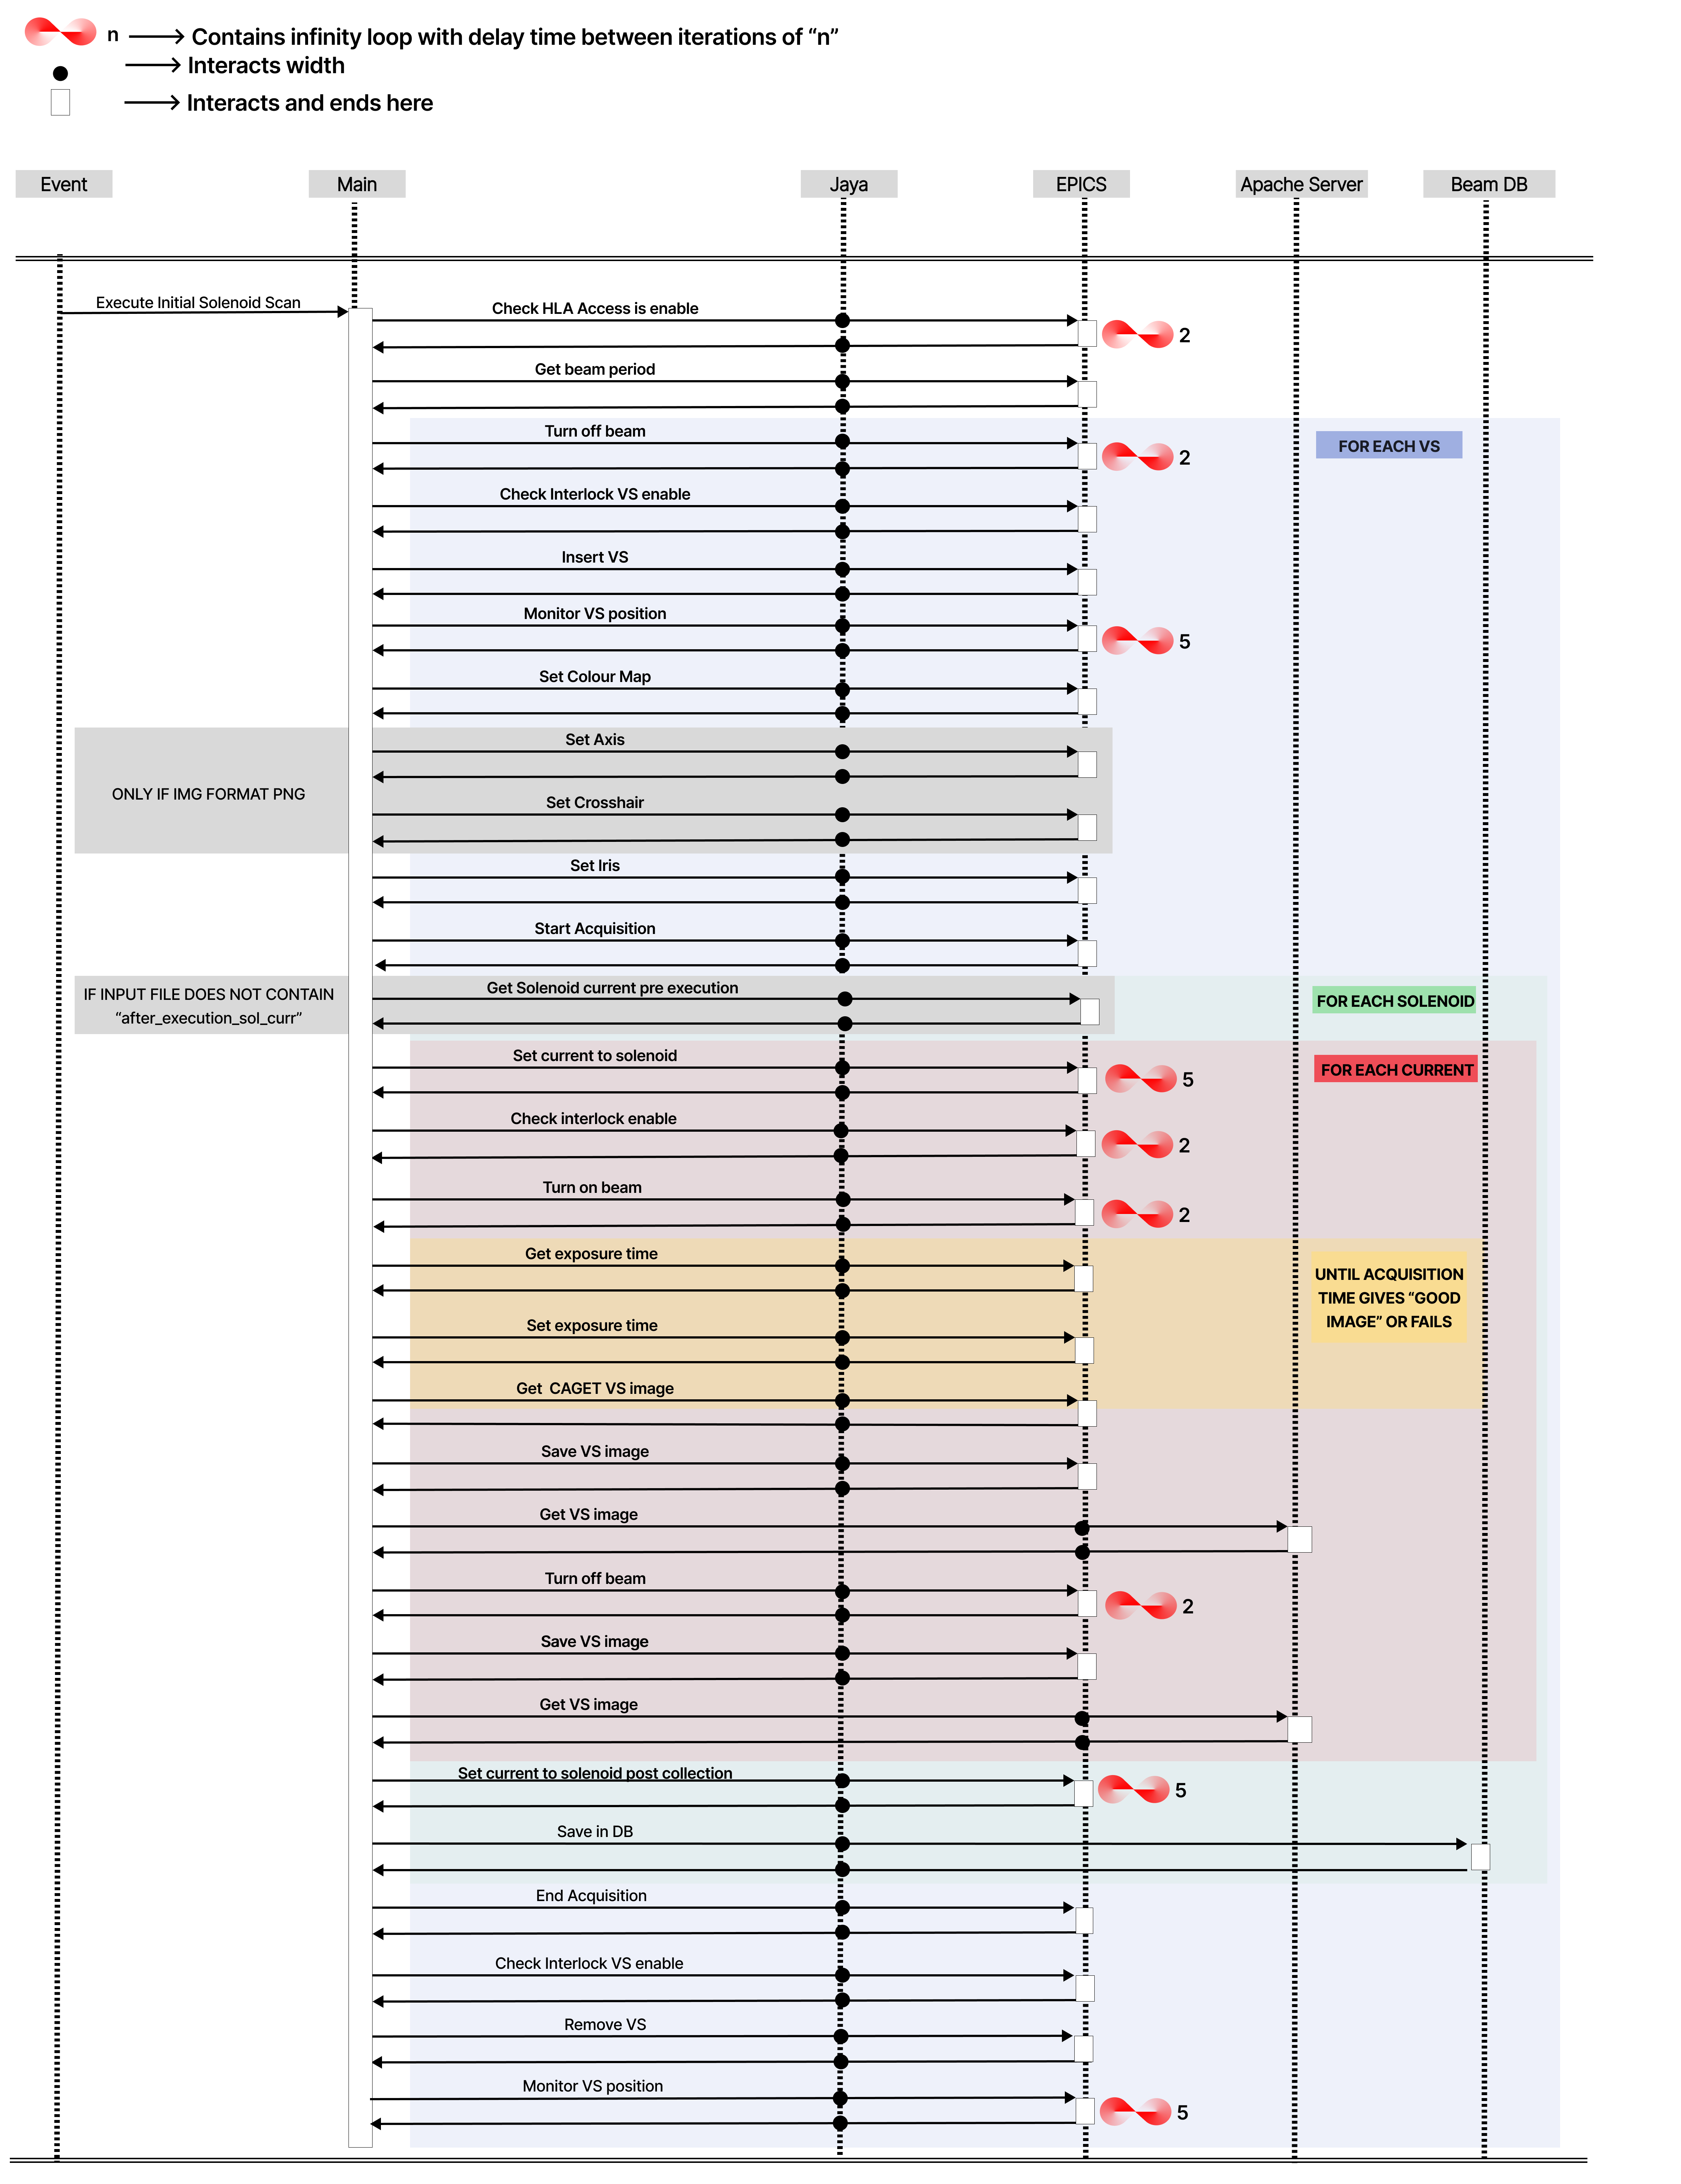
\includegraphics[width=\linewidth]{images/init_conditions.png}
  \caption{Request diagram for all interactions to collect a VS image for online init$\_$scan modality.}
  \label{fig:99}
\end{figure} 
\newpage
\section{Esnapshot execution diagram} \label{appendix:esnapshot_exe}
\begin{figure}[!h]  
  \centering
  % 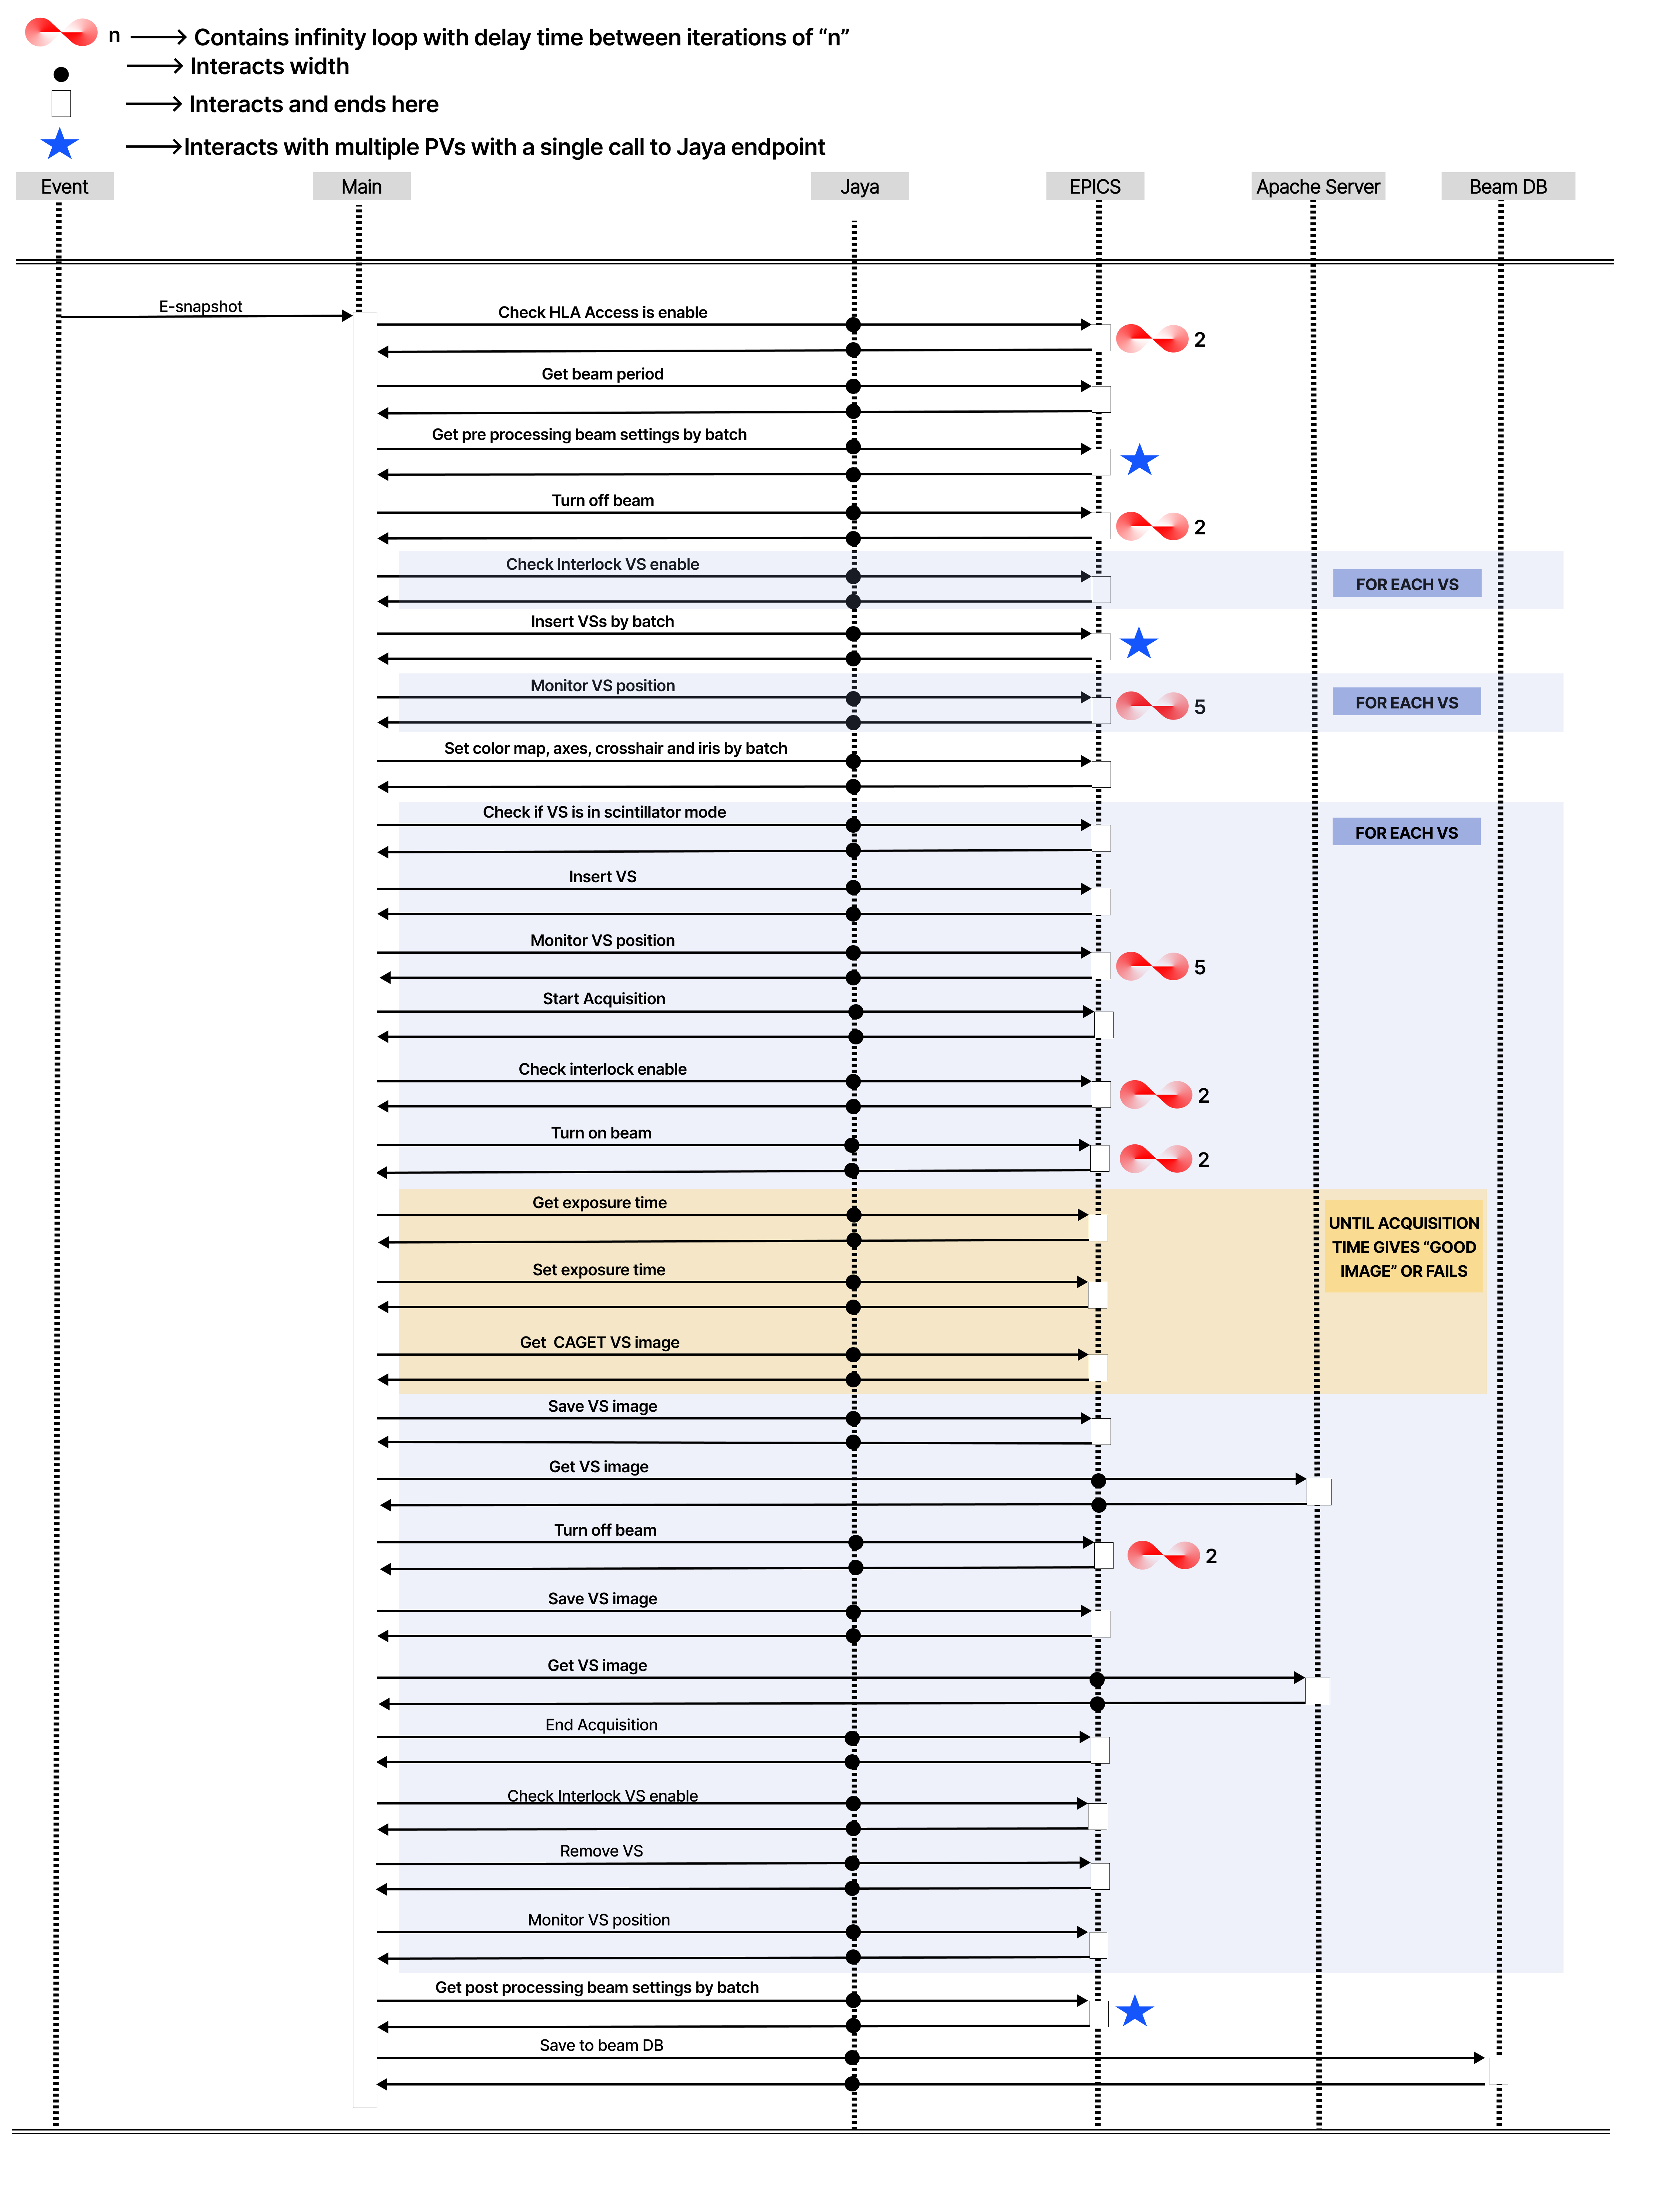
\includegraphics[width=\linewidth]{Images/e_snapshot.png}
  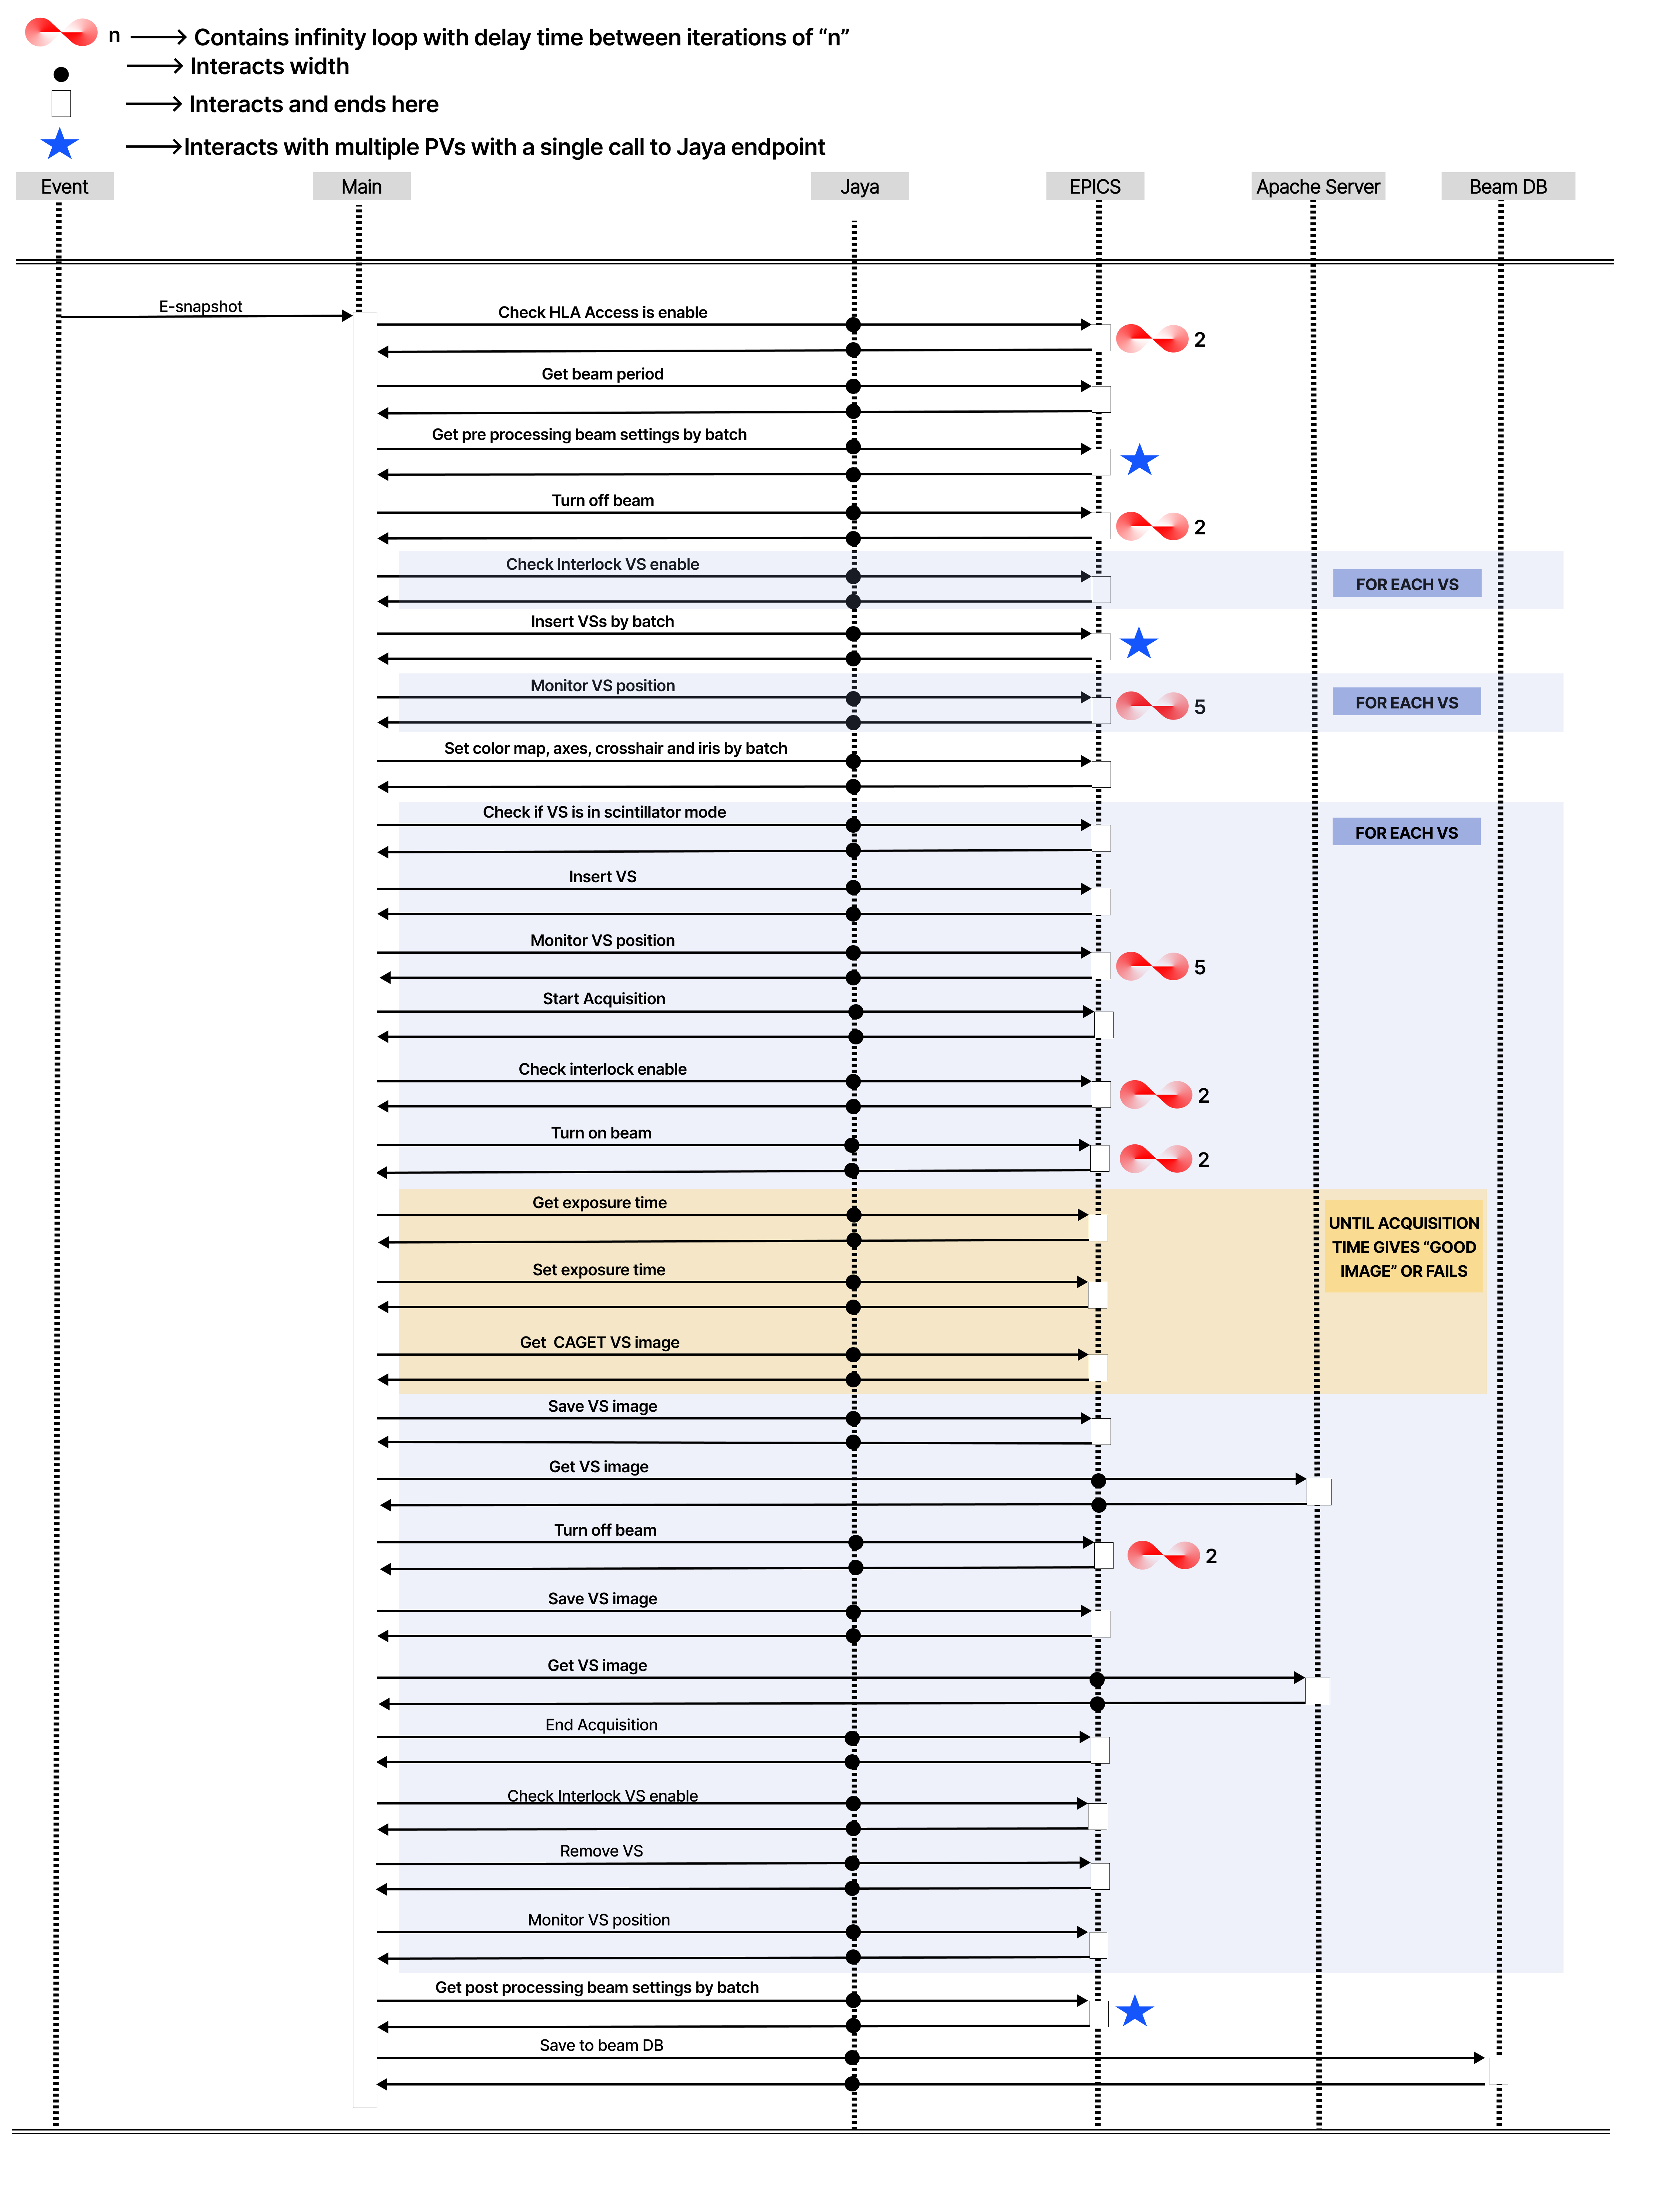
\includegraphics[width=\linewidth]{images/e_snapshot.png}
  \caption{Request diagram for all interactions to collect a VS image for online esnapshot modality.}
  \label{fig:100}
\end{figure} 

\end{document}
